% Options for packages loaded elsewhere
\PassOptionsToPackage{unicode}{hyperref}
\PassOptionsToPackage{hyphens}{url}
%
\documentclass[
]{article}
\usepackage{amsmath,amssymb}
\usepackage{iftex}
\ifPDFTeX
  \usepackage[T1]{fontenc}
  \usepackage[utf8]{inputenc}
  \usepackage{textcomp} % provide euro and other symbols
\else % if luatex or xetex
  \usepackage{unicode-math} % this also loads fontspec
  \defaultfontfeatures{Scale=MatchLowercase}
  \defaultfontfeatures[\rmfamily]{Ligatures=TeX,Scale=1}
\fi
\usepackage{lmodern}
\ifPDFTeX\else
  % xetex/luatex font selection
  \setmainfont[]{Arial}
\fi
% Use upquote if available, for straight quotes in verbatim environments
\IfFileExists{upquote.sty}{\usepackage{upquote}}{}
\IfFileExists{microtype.sty}{% use microtype if available
  \usepackage[]{microtype}
  \UseMicrotypeSet[protrusion]{basicmath} % disable protrusion for tt fonts
}{}
\makeatletter
\@ifundefined{KOMAClassName}{% if non-KOMA class
  \IfFileExists{parskip.sty}{%
    \usepackage{parskip}
  }{% else
    \setlength{\parindent}{0pt}
    \setlength{\parskip}{6pt plus 2pt minus 1pt}}
}{% if KOMA class
  \KOMAoptions{parskip=half}}
\makeatother
\usepackage{xcolor}
\usepackage[margin=1in]{geometry}
\usepackage{color}
\usepackage{fancyvrb}
\newcommand{\VerbBar}{|}
\newcommand{\VERB}{\Verb[commandchars=\\\{\}]}
\DefineVerbatimEnvironment{Highlighting}{Verbatim}{commandchars=\\\{\}}
% Add ',fontsize=\small' for more characters per line
\usepackage{framed}
\definecolor{shadecolor}{RGB}{248,248,248}
\newenvironment{Shaded}{\begin{snugshade}}{\end{snugshade}}
\newcommand{\AlertTok}[1]{\textcolor[rgb]{0.94,0.16,0.16}{#1}}
\newcommand{\AnnotationTok}[1]{\textcolor[rgb]{0.56,0.35,0.01}{\textbf{\textit{#1}}}}
\newcommand{\AttributeTok}[1]{\textcolor[rgb]{0.13,0.29,0.53}{#1}}
\newcommand{\BaseNTok}[1]{\textcolor[rgb]{0.00,0.00,0.81}{#1}}
\newcommand{\BuiltInTok}[1]{#1}
\newcommand{\CharTok}[1]{\textcolor[rgb]{0.31,0.60,0.02}{#1}}
\newcommand{\CommentTok}[1]{\textcolor[rgb]{0.56,0.35,0.01}{\textit{#1}}}
\newcommand{\CommentVarTok}[1]{\textcolor[rgb]{0.56,0.35,0.01}{\textbf{\textit{#1}}}}
\newcommand{\ConstantTok}[1]{\textcolor[rgb]{0.56,0.35,0.01}{#1}}
\newcommand{\ControlFlowTok}[1]{\textcolor[rgb]{0.13,0.29,0.53}{\textbf{#1}}}
\newcommand{\DataTypeTok}[1]{\textcolor[rgb]{0.13,0.29,0.53}{#1}}
\newcommand{\DecValTok}[1]{\textcolor[rgb]{0.00,0.00,0.81}{#1}}
\newcommand{\DocumentationTok}[1]{\textcolor[rgb]{0.56,0.35,0.01}{\textbf{\textit{#1}}}}
\newcommand{\ErrorTok}[1]{\textcolor[rgb]{0.64,0.00,0.00}{\textbf{#1}}}
\newcommand{\ExtensionTok}[1]{#1}
\newcommand{\FloatTok}[1]{\textcolor[rgb]{0.00,0.00,0.81}{#1}}
\newcommand{\FunctionTok}[1]{\textcolor[rgb]{0.13,0.29,0.53}{\textbf{#1}}}
\newcommand{\ImportTok}[1]{#1}
\newcommand{\InformationTok}[1]{\textcolor[rgb]{0.56,0.35,0.01}{\textbf{\textit{#1}}}}
\newcommand{\KeywordTok}[1]{\textcolor[rgb]{0.13,0.29,0.53}{\textbf{#1}}}
\newcommand{\NormalTok}[1]{#1}
\newcommand{\OperatorTok}[1]{\textcolor[rgb]{0.81,0.36,0.00}{\textbf{#1}}}
\newcommand{\OtherTok}[1]{\textcolor[rgb]{0.56,0.35,0.01}{#1}}
\newcommand{\PreprocessorTok}[1]{\textcolor[rgb]{0.56,0.35,0.01}{\textit{#1}}}
\newcommand{\RegionMarkerTok}[1]{#1}
\newcommand{\SpecialCharTok}[1]{\textcolor[rgb]{0.81,0.36,0.00}{\textbf{#1}}}
\newcommand{\SpecialStringTok}[1]{\textcolor[rgb]{0.31,0.60,0.02}{#1}}
\newcommand{\StringTok}[1]{\textcolor[rgb]{0.31,0.60,0.02}{#1}}
\newcommand{\VariableTok}[1]{\textcolor[rgb]{0.00,0.00,0.00}{#1}}
\newcommand{\VerbatimStringTok}[1]{\textcolor[rgb]{0.31,0.60,0.02}{#1}}
\newcommand{\WarningTok}[1]{\textcolor[rgb]{0.56,0.35,0.01}{\textbf{\textit{#1}}}}
\usepackage{graphicx}
\makeatletter
\def\maxwidth{\ifdim\Gin@nat@width>\linewidth\linewidth\else\Gin@nat@width\fi}
\def\maxheight{\ifdim\Gin@nat@height>\textheight\textheight\else\Gin@nat@height\fi}
\makeatother
% Scale images if necessary, so that they will not overflow the page
% margins by default, and it is still possible to overwrite the defaults
% using explicit options in \includegraphics[width, height, ...]{}
\setkeys{Gin}{width=\maxwidth,height=\maxheight,keepaspectratio}
% Set default figure placement to htbp
\makeatletter
\def\fps@figure{htbp}
\makeatother
\setlength{\emergencystretch}{3em} % prevent overfull lines
\providecommand{\tightlist}{%
  \setlength{\itemsep}{0pt}\setlength{\parskip}{0pt}}
\setcounter{secnumdepth}{-\maxdimen} % remove section numbering
\ifLuaTeX
  \usepackage{selnolig}  % disable illegal ligatures
\fi
\IfFileExists{bookmark.sty}{\usepackage{bookmark}}{\usepackage{hyperref}}
\IfFileExists{xurl.sty}{\usepackage{xurl}}{} % add URL line breaks if available
\urlstyle{same}
\hypersetup{
  pdftitle={Analysis of BGC content across phylum Cyanobacteriota},
  hidelinks,
  pdfcreator={LaTeX via pandoc}}

\title{Analysis of BGC content across phylum Cyanobacteriota}
\author{}
\date{\vspace{-2.5em}}

\begin{document}
\maketitle

\hypertarget{setup}{%
\section{Setup}\label{setup}}

\hypertarget{read-in-data}{%
\subsection{Read in data}\label{read-in-data}}

\begin{Shaded}
\begin{Highlighting}[]
\CommentTok{\# Map antiSMASH classes to their categories}
\NormalTok{bgc\_class }\OtherTok{\textless{}{-}} \FunctionTok{read\_tsv}\NormalTok{(}\StringTok{"./data/2025{-}01{-}16{-}1256{-}bgc\_class\_ref.tsv"}\NormalTok{) }\SpecialCharTok{\%\textgreater{}\%} \FunctionTok{select}\NormalTok{(}\SpecialCharTok{!}\NormalTok{owner\_id)}
\NormalTok{class\_to\_cat }\OtherTok{\textless{}{-}}\NormalTok{ bgc\_class}\SpecialCharTok{$}\NormalTok{bgc\_category}
\FunctionTok{names}\NormalTok{(class\_to\_cat) }\OtherTok{\textless{}{-}}\NormalTok{ bgc\_class}\SpecialCharTok{$}\NormalTok{class\_name}

\CommentTok{\# NCBI Taxonomy data for Cyanobacteriota assemblies}
\NormalTok{cyano\_asm\_tax }\OtherTok{\textless{}{-}} \FunctionTok{read\_tsv}\NormalTok{(}\StringTok{"data/cyano\_asm\_tax.tsv"}\NormalTok{)}

\CommentTok{\# From SMC: All antiSMASH \textquotesingle{}region\textquotesingle{}s for Cyanobacteriota genomes}
\NormalTok{regions }\OtherTok{\textless{}{-}} \FunctionTok{read\_tsv}\NormalTok{(}\StringTok{"./data/2025{-}02{-}26{-}1456{-}cyano\_as\_regions.tsv"}\NormalTok{)}

\CommentTok{\# Table of NCBI assemblies at "chromosome" or "complete" quality levels}
\NormalTok{ncbi\_hiq\_meta }\OtherTok{\textless{}{-}} \FunctionTok{read\_tsv}\NormalTok{(}\StringTok{"data/ncbi\_cyano\_HiQualityGenomes\_metadata.tsv"}\NormalTok{)}
\end{Highlighting}
\end{Shaded}

\hypertarget{clean-data}{%
\subsection{Clean data}\label{clean-data}}

\begin{Shaded}
\begin{Highlighting}[]
\CommentTok{\# Convert BGC \textquotesingle{}class\textquotesingle{} to vector, add in BGC \textquotesingle{}category\textquotesingle{} as vector, order levels of classes and categories}
\NormalTok{regions }\OtherTok{\textless{}{-}}\NormalTok{ regions }\SpecialCharTok{\%\textgreater{}\%}
  \FunctionTok{mutate}\NormalTok{(}\AttributeTok{classes =} \FunctionTok{map}\NormalTok{(region\_class, }\ControlFlowTok{function}\NormalTok{(class\_string) \{}
\NormalTok{    (}
      \ControlFlowTok{if}\NormalTok{ (}\FunctionTok{str\_starts}\NormalTok{(class\_string, }\FunctionTok{fixed}\NormalTok{(}\StringTok{"["}\NormalTok{))) \{}
        \FunctionTok{fromJSON}\NormalTok{(class\_string)}
\NormalTok{      \} }\ControlFlowTok{else}\NormalTok{ \{}
        \FunctionTok{c}\NormalTok{(class\_string)}
\NormalTok{      \}}
\NormalTok{    )}
\NormalTok{  \})) }\SpecialCharTok{\%\textgreater{}\%}
  \FunctionTok{mutate}\NormalTok{(}\AttributeTok{categories =}\NormalTok{ classes }\SpecialCharTok{\%\textgreater{}\%} \FunctionTok{map}\NormalTok{(}\ControlFlowTok{function}\NormalTok{(cls\_vec) \{}
\NormalTok{    (}
      \FunctionTok{map\_vec}\NormalTok{(cls\_vec, }\ControlFlowTok{function}\NormalTok{(cls\_str) class\_to\_cat[[cls\_str]]) }\SpecialCharTok{\%\textgreater{}\%} \FunctionTok{unique}\NormalTok{() }\SpecialCharTok{\%\textgreater{}\%} \FunctionTok{sort}\NormalTok{())}
\NormalTok{  \})) }\SpecialCharTok{\%\textgreater{}\%}
  \FunctionTok{mutate}\NormalTok{(}\AttributeTok{cats\_str =}\NormalTok{ categories }\SpecialCharTok{\%\textgreater{}\%} \FunctionTok{map\_chr}\NormalTok{(}\ControlFlowTok{function}\NormalTok{(x) }\FunctionTok{str\_flatten}\NormalTok{(x, }\AttributeTok{collapse =} \StringTok{", "}\NormalTok{))) }\SpecialCharTok{\%\textgreater{}\%}
  \FunctionTok{add\_count}\NormalTok{(cats\_str) }\SpecialCharTok{\%\textgreater{}\%}
  \FunctionTok{mutate}\NormalTok{(}
    \AttributeTok{cats\_str =}\NormalTok{ forcats}\SpecialCharTok{::}\FunctionTok{fct\_reorder}\NormalTok{(cats\_str, }\FunctionTok{desc}\NormalTok{(n)),}
    \AttributeTok{class\_str =}\NormalTok{ classes }\SpecialCharTok{\%\textgreater{}\%} \FunctionTok{map\_chr}\NormalTok{(}\ControlFlowTok{function}\NormalTok{(x) }\FunctionTok{str\_flatten}\NormalTok{(x, }\AttributeTok{collapse =} \StringTok{", "}\NormalTok{))}
\NormalTok{  )}

\NormalTok{regions}
\end{Highlighting}
\end{Shaded}

\begin{verbatim}
## # A tibble: 32,112 x 26
##    region_gene_id bgc_id region_length contig_name region_start_nt region_end_nt
##             <dbl>  <dbl>         <dbl> <chr>                 <dbl>         <dbl>
##  1      394444400 2.05e6         20822 NZ_KK07376~         1448721       1469542
##  2      427693693 2.21e6          6191 NZ_NMQI010~               1          6191
##  3      427830749 2.21e6         41152 NZ_NJHU010~           20319         61470
##  4      427867799 2.21e6         29334 NZ_NJHW010~            5515         34848
##  5      427879170 2.21e6          5638 NZ_NJHW010~               1          5638
##  6      442232549 2.29e6         27366 NZ_VIKX010~               1         27366
##  7      442951361 2.29e6         61852 NZ_BJCK010~          121631        183482
##  8      444447386 2.30e6         21923 NZ_WVIC010~           13038         34960
##  9      445057742 2.31e6         40108 NZ_JAAGOG0~           26815         66922
## 10      446681012 2.31e6         35928 NZ_QMEA010~               1         35928
## # i 32,102 more rows
## # i 20 more variables: bgc_annotation_id <dbl>, region_class <chr>,
## #   region_category <lgl>, contig_edge <lgl>, smc_id <dbl>, accession_id <chr>,
## #   size_bp <dbl>, n_scaffolds <dbl>, data_source_description <chr>,
## #   tax_phylum <chr>, tax_class <chr>, tax_order <chr>, tax_family <chr>,
## #   tax_genus <chr>, tax_species <chr>, classes <list>, categories <list>,
## #   cats_str <fct>, n <int>, class_str <chr>
\end{verbatim}

\hypertarget{explore-data}{%
\subsection{Explore data}\label{explore-data}}

The repetitive composition of many BGCs makes them a challenge during
genome assembly, resulting in over-inflation of BGC counts when BGCs are
split between the ends of two different contigs. Focusing on
high-quality genomes can therefore ensure a higher-quality dataset.

\hypertarget{how-fragmented-are-the-full-set-of-genomes-and-how-does-that-impact-bgc-counts}{%
\subsubsection{How fragmented are the full set of genomes, and how does
that impact BGC
counts?}\label{how-fragmented-are-the-full-set-of-genomes-and-how-does-that-impact-bgc-counts}}

\begin{Shaded}
\begin{Highlighting}[]
\NormalTok{regions }\SpecialCharTok{\%\textgreater{}\%}
  \FunctionTok{group\_by}\NormalTok{(smc\_id, n\_scaffolds, contig\_edge) }\SpecialCharTok{\%\textgreater{}\%}
  \FunctionTok{summarize}\NormalTok{(}\AttributeTok{n\_bgcs =} \FunctionTok{n}\NormalTok{()) }\SpecialCharTok{\%\textgreater{}\%}
  \FunctionTok{ungroup}\NormalTok{() }\SpecialCharTok{\%\textgreater{}\%}
  \FunctionTok{ggplot}\NormalTok{(}\FunctionTok{aes}\NormalTok{(}\AttributeTok{x =}\NormalTok{ n\_scaffolds, }\AttributeTok{y =}\NormalTok{ n\_bgcs)) }\SpecialCharTok{+}
  \FunctionTok{stat\_bin\_hex}\NormalTok{(}\AttributeTok{bins =} \DecValTok{50}\NormalTok{) }\SpecialCharTok{+}
  \FunctionTok{scale\_x\_log10}\NormalTok{(}\AttributeTok{breaks =} \FunctionTok{breaks\_log}\NormalTok{()) }\SpecialCharTok{+}
  \FunctionTok{guides}\NormalTok{(}\AttributeTok{fill =} \FunctionTok{guide\_colorbar}\NormalTok{(}\AttributeTok{title =} \StringTok{"\# Genomes"}\NormalTok{)) }\SpecialCharTok{+}
  \FunctionTok{facet\_wrap}\NormalTok{(. }\SpecialCharTok{\textasciitilde{}}\NormalTok{ contig\_edge, }\AttributeTok{ncol =} \DecValTok{1}\NormalTok{, }\AttributeTok{labeller =} \FunctionTok{as\_labeller}\NormalTok{(}\FunctionTok{c}\NormalTok{(}\StringTok{"FALSE"} \OtherTok{=} \StringTok{"BGCs not on contig edge"}\NormalTok{, }\StringTok{"TRUE"} \OtherTok{=} \StringTok{"BGCs on contig edge"}\NormalTok{))) }\SpecialCharTok{+}
  \FunctionTok{theme\_bw}\NormalTok{() }\SpecialCharTok{+}
  \FunctionTok{ggtitle}\NormalTok{(}\StringTok{"Fragmented genomes have inflated BGC counts"}\NormalTok{, }\AttributeTok{subtitle =} \StringTok{"Full dataset"}\NormalTok{)}
\end{Highlighting}
\end{Shaded}

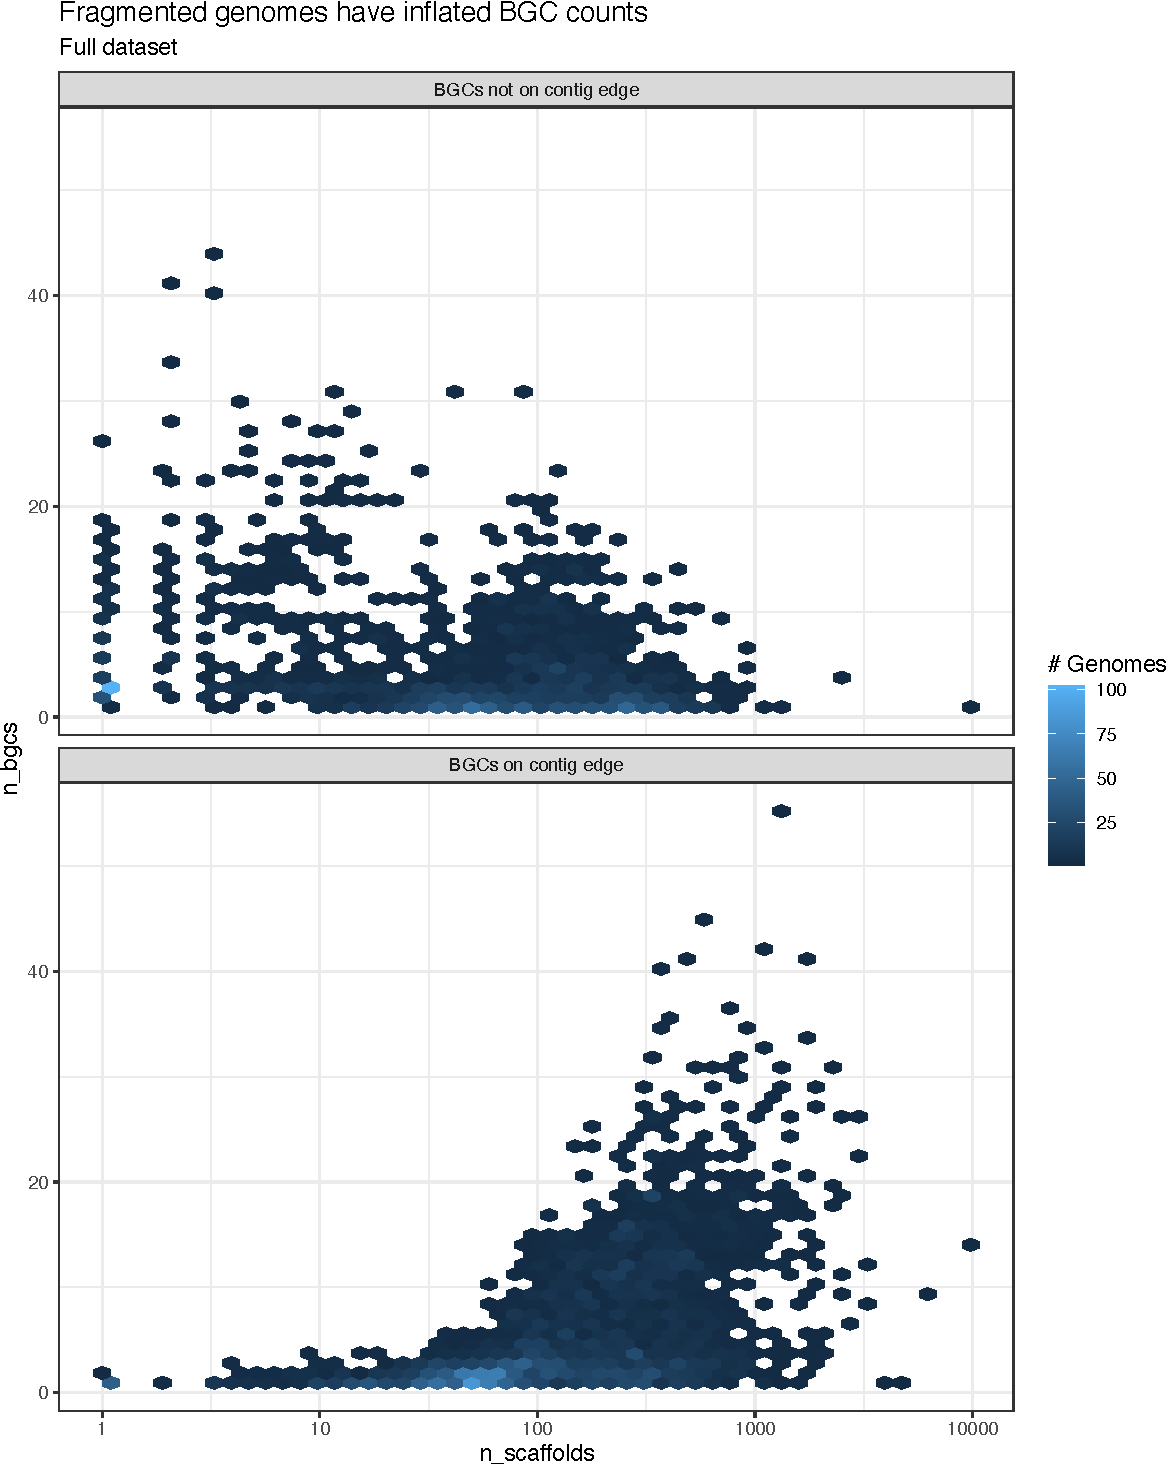
\includegraphics{analysis_files/figure-latex/unnamed-chunk-3-1.pdf} This
figure depicts the number of BGCs against the number of scaffolds in a
genome. To help avoid overplotting (i.e.~many overlapping data points
misrepresenting the distribution of the data), the colors of each spot
in the figure correspond to how many data points overlap at those
coordinates.

\hypertarget{how-does-the-proportion-of-bgcs-offon-a-contig-edge-change-if-we-filter-for-high-quality-genomes-in-different-ways}{%
\subsubsection{How does the proportion of BGCs off/on a contig edge
change if we filter for high-quality genomes in different
ways?}\label{how-does-the-proportion-of-bgcs-offon-a-contig-edge-change-if-we-filter-for-high-quality-genomes-in-different-ways}}

\begin{Shaded}
\begin{Highlighting}[]
\NormalTok{filters\_df }\OtherTok{\textless{}{-}} \FunctionTok{bind\_rows}\NormalTok{(}
\NormalTok{  regions }\SpecialCharTok{\%\textgreater{}\%}
    \FunctionTok{group\_by}\NormalTok{(contig\_edge) }\SpecialCharTok{\%\textgreater{}\%}
    \FunctionTok{summarize}\NormalTok{(}\AttributeTok{filter =} \StringTok{"Unfiltered"}\NormalTok{, }\AttributeTok{n =} \FunctionTok{n}\NormalTok{()) }\SpecialCharTok{\%\textgreater{}\%}
    \FunctionTok{ungroup}\NormalTok{() }\SpecialCharTok{\%\textgreater{}\%}
    \FunctionTok{mutate}\NormalTok{(}\AttributeTok{pct =} \DecValTok{100} \SpecialCharTok{*}\NormalTok{ n }\SpecialCharTok{/} \FunctionTok{sum}\NormalTok{(n)),}
\NormalTok{  regions }\SpecialCharTok{\%\textgreater{}\%}
    \FunctionTok{semi\_join}\NormalTok{(ncbi\_hiq\_meta, }\AttributeTok{by =} \FunctionTok{join\_by}\NormalTok{(accession\_id }\SpecialCharTok{==} \StringTok{\textasciigrave{}}\AttributeTok{Assembly Accession}\StringTok{\textasciigrave{}}\NormalTok{)) }\SpecialCharTok{\%\textgreater{}\%}
    \FunctionTok{group\_by}\NormalTok{(contig\_edge) }\SpecialCharTok{\%\textgreater{}\%}
    \FunctionTok{summarize}\NormalTok{(}\AttributeTok{filter =} \StringTok{"Complete/Chromosome"}\NormalTok{, }\AttributeTok{n =} \FunctionTok{n}\NormalTok{()) }\SpecialCharTok{\%\textgreater{}\%}
    \FunctionTok{mutate}\NormalTok{(}\AttributeTok{pct =} \DecValTok{100} \SpecialCharTok{*}\NormalTok{ n }\SpecialCharTok{/} \FunctionTok{sum}\NormalTok{(n)),}
\NormalTok{  regions }\SpecialCharTok{\%\textgreater{}\%}
    \FunctionTok{filter}\NormalTok{(n\_scaffolds }\SpecialCharTok{\textless{}} \DecValTok{10}\NormalTok{) }\SpecialCharTok{\%\textgreater{}\%}
    \FunctionTok{group\_by}\NormalTok{(contig\_edge) }\SpecialCharTok{\%\textgreater{}\%}
    \FunctionTok{summarize}\NormalTok{(}\AttributeTok{filter =} \StringTok{"\textless{} 10 Scaffolds"}\NormalTok{, }\AttributeTok{n =} \FunctionTok{n}\NormalTok{()) }\SpecialCharTok{\%\textgreater{}\%}
    \FunctionTok{mutate}\NormalTok{(}\AttributeTok{pct =} \DecValTok{100} \SpecialCharTok{*}\NormalTok{ n }\SpecialCharTok{/} \FunctionTok{sum}\NormalTok{(n)),}
\NormalTok{  regions }\SpecialCharTok{\%\textgreater{}\%}
    \FunctionTok{filter}\NormalTok{(n\_scaffolds }\SpecialCharTok{\textless{}} \DecValTok{20}\NormalTok{) }\SpecialCharTok{\%\textgreater{}\%}
    \FunctionTok{group\_by}\NormalTok{(contig\_edge) }\SpecialCharTok{\%\textgreater{}\%}
    \FunctionTok{summarize}\NormalTok{(}\AttributeTok{filter =} \StringTok{"\textless{} 20 Scaffolds"}\NormalTok{, }\AttributeTok{n =} \FunctionTok{n}\NormalTok{()) }\SpecialCharTok{\%\textgreater{}\%}
    \FunctionTok{mutate}\NormalTok{(}\AttributeTok{pct =} \DecValTok{100} \SpecialCharTok{*}\NormalTok{ n }\SpecialCharTok{/} \FunctionTok{sum}\NormalTok{(n)),}
\NormalTok{  regions }\SpecialCharTok{\%\textgreater{}\%}
    \FunctionTok{filter}\NormalTok{(n\_scaffolds }\SpecialCharTok{\textless{}} \DecValTok{25}\NormalTok{) }\SpecialCharTok{\%\textgreater{}\%}
    \FunctionTok{group\_by}\NormalTok{(contig\_edge) }\SpecialCharTok{\%\textgreater{}\%}
    \FunctionTok{summarize}\NormalTok{(}\AttributeTok{filter =} \StringTok{"\textless{} 25 Scaffolds"}\NormalTok{, }\AttributeTok{n =} \FunctionTok{n}\NormalTok{()) }\SpecialCharTok{\%\textgreater{}\%}
    \FunctionTok{mutate}\NormalTok{(}\AttributeTok{pct =} \DecValTok{100} \SpecialCharTok{*}\NormalTok{ n }\SpecialCharTok{/} \FunctionTok{sum}\NormalTok{(n)),}
\NormalTok{  regions }\SpecialCharTok{\%\textgreater{}\%}
    \FunctionTok{filter}\NormalTok{(n\_scaffolds }\SpecialCharTok{\textless{}} \DecValTok{30}\NormalTok{) }\SpecialCharTok{\%\textgreater{}\%}
    \FunctionTok{group\_by}\NormalTok{(contig\_edge) }\SpecialCharTok{\%\textgreater{}\%}
    \FunctionTok{summarize}\NormalTok{(}\AttributeTok{filter =} \StringTok{"\textless{} 30 Scaffolds"}\NormalTok{, }\AttributeTok{n =} \FunctionTok{n}\NormalTok{()) }\SpecialCharTok{\%\textgreater{}\%}
    \FunctionTok{mutate}\NormalTok{(}\AttributeTok{pct =} \DecValTok{100} \SpecialCharTok{*}\NormalTok{ n }\SpecialCharTok{/} \FunctionTok{sum}\NormalTok{(n)),}
\NormalTok{  regions }\SpecialCharTok{\%\textgreater{}\%}
    \FunctionTok{filter}\NormalTok{(n\_scaffolds }\SpecialCharTok{\textless{}} \DecValTok{50}\NormalTok{) }\SpecialCharTok{\%\textgreater{}\%}
    \FunctionTok{group\_by}\NormalTok{(contig\_edge) }\SpecialCharTok{\%\textgreater{}\%}
    \FunctionTok{summarize}\NormalTok{(}\AttributeTok{filter =} \StringTok{"\textless{} 50 Scaffolds"}\NormalTok{, }\AttributeTok{n =} \FunctionTok{n}\NormalTok{()) }\SpecialCharTok{\%\textgreater{}\%}
    \FunctionTok{mutate}\NormalTok{(}\AttributeTok{pct =} \DecValTok{100} \SpecialCharTok{*}\NormalTok{ n }\SpecialCharTok{/} \FunctionTok{sum}\NormalTok{(n)),}
\NormalTok{  regions }\SpecialCharTok{\%\textgreater{}\%}
    \FunctionTok{filter}\NormalTok{(n\_scaffolds }\SpecialCharTok{\textless{}} \DecValTok{100}\NormalTok{) }\SpecialCharTok{\%\textgreater{}\%}
    \FunctionTok{group\_by}\NormalTok{(contig\_edge) }\SpecialCharTok{\%\textgreater{}\%}
    \FunctionTok{summarize}\NormalTok{(}\AttributeTok{filter =} \StringTok{"\textless{} 100 Scaffolds"}\NormalTok{, }\AttributeTok{n =} \FunctionTok{n}\NormalTok{()) }\SpecialCharTok{\%\textgreater{}\%}
    \FunctionTok{mutate}\NormalTok{(}\AttributeTok{pct =} \DecValTok{100} \SpecialCharTok{*}\NormalTok{ n }\SpecialCharTok{/} \FunctionTok{sum}\NormalTok{(n)),}
\NormalTok{)}

\FunctionTok{ggplot}\NormalTok{(filters\_df, }\FunctionTok{aes}\NormalTok{(}\AttributeTok{x =}\NormalTok{ filter, }\AttributeTok{y =}\NormalTok{ n)) }\SpecialCharTok{+}
  \FunctionTok{geom\_col}\NormalTok{(}\FunctionTok{aes}\NormalTok{(}\AttributeTok{fill =} \FunctionTok{fct\_rev}\NormalTok{(}\FunctionTok{as\_factor}\NormalTok{(contig\_edge))), }\AttributeTok{position =} \FunctionTok{position\_stack}\NormalTok{()) }\SpecialCharTok{+}
  \FunctionTok{geom\_text}\NormalTok{(}\FunctionTok{aes}\NormalTok{(}\AttributeTok{y =}\NormalTok{ n, }\AttributeTok{label =} \FunctionTok{sprintf}\NormalTok{(}\StringTok{"\%1.1f\%\%"}\NormalTok{, pct)), }\AttributeTok{data =}\NormalTok{ filters\_df }\SpecialCharTok{\%\textgreater{}\%} \FunctionTok{filter}\NormalTok{(contig\_edge }\SpecialCharTok{==} \ConstantTok{FALSE}\NormalTok{), }\AttributeTok{hjust =} \SpecialCharTok{{-}}\FloatTok{0.1}\NormalTok{) }\SpecialCharTok{+}
  \FunctionTok{scale\_x\_discrete}\NormalTok{(}\AttributeTok{name =} \StringTok{""}\NormalTok{, }\AttributeTok{limits =} \FunctionTok{c}\NormalTok{(}\StringTok{"Unfiltered"}\NormalTok{, }\StringTok{"\textless{} 100 Scaffolds"}\NormalTok{, }\StringTok{"\textless{} 50 Scaffolds"}\NormalTok{, }\StringTok{"\textless{} 30 Scaffolds"}\NormalTok{, }\StringTok{"\textless{} 25 Scaffolds"}\NormalTok{, }\StringTok{"\textless{} 20 Scaffolds"}\NormalTok{, }\StringTok{"\textless{} 10 Scaffolds"}\NormalTok{, }\StringTok{"Complete/Chromosome"}\NormalTok{)) }\SpecialCharTok{+}
  \FunctionTok{scale\_y\_continuous}\NormalTok{(}\AttributeTok{name =} \StringTok{"Number of BGCs"}\NormalTok{, }\AttributeTok{labels =} \FunctionTok{label\_comma}\NormalTok{()) }\SpecialCharTok{+}
  \FunctionTok{scale\_fill\_manual}\NormalTok{(}\AttributeTok{name =} \StringTok{"BGC on contig edge"}\NormalTok{, }\AttributeTok{values =} \FunctionTok{c}\NormalTok{(}\StringTok{"gray80"}\NormalTok{, }\StringTok{"black"}\NormalTok{)) }\SpecialCharTok{+}
  \FunctionTok{theme\_classic}\NormalTok{() }\SpecialCharTok{+}
  \FunctionTok{coord\_flip}\NormalTok{()}
\end{Highlighting}
\end{Shaded}

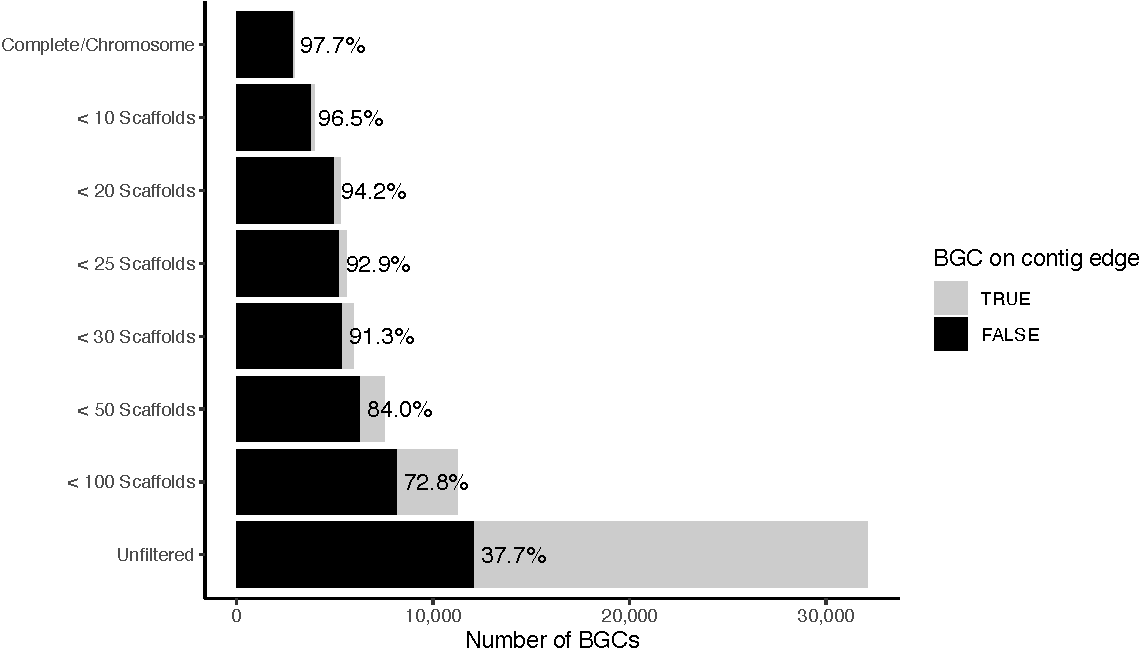
\includegraphics{analysis_files/figure-latex/unnamed-chunk-4-1.pdf} This
figure depicts the counts of BGCs that are on a contig edge vs.~those
that are not, depending on how we define what a ``high-quality genome''
is. \texttt{Complete/Chromosome} refers to the genomes at the
``Complete'' or ``Chromosome'' assembly levels on NCBI.

Based on this figure, and to be most conservative in this analysis, we
will be going with the most restrictive criteria -- using only genomes
of ``Chromosome'' or ``Complete'' assembly quality as listed on NCBI.

\hypertarget{filter-the-dataset-to-high-quality-genomes}{%
\subsection{Filter the dataset to high-quality
genomes}\label{filter-the-dataset-to-high-quality-genomes}}

Repeat the figure from above, and we should see that most BGCs are not
on a contig edge.

\begin{Shaded}
\begin{Highlighting}[]
\NormalTok{regions }\OtherTok{\textless{}{-}}\NormalTok{ regions }\SpecialCharTok{\%\textgreater{}\%}
  \FunctionTok{semi\_join}\NormalTok{(ncbi\_hiq\_meta, }\AttributeTok{by =} \FunctionTok{join\_by}\NormalTok{(accession\_id }\SpecialCharTok{==} \StringTok{\textasciigrave{}}\AttributeTok{Assembly Accession}\StringTok{\textasciigrave{}}\NormalTok{))}

\NormalTok{regions }\SpecialCharTok{\%\textgreater{}\%}
  \FunctionTok{group\_by}\NormalTok{(smc\_id, tax\_genus, n\_scaffolds, contig\_edge) }\SpecialCharTok{\%\textgreater{}\%}
  \FunctionTok{summarize}\NormalTok{(}\AttributeTok{n\_bgcs =} \FunctionTok{n}\NormalTok{()) }\SpecialCharTok{\%\textgreater{}\%}
  \FunctionTok{ggplot}\NormalTok{(}\FunctionTok{aes}\NormalTok{(}\AttributeTok{x =}\NormalTok{ n\_scaffolds, }\AttributeTok{y =}\NormalTok{ n\_bgcs)) }\SpecialCharTok{+}
  \FunctionTok{stat\_bin\_hex}\NormalTok{(}\AttributeTok{bins =} \DecValTok{50}\NormalTok{) }\SpecialCharTok{+}
  \FunctionTok{facet\_wrap}\NormalTok{(. }\SpecialCharTok{\textasciitilde{}}\NormalTok{ contig\_edge, }\AttributeTok{ncol =} \DecValTok{1}\NormalTok{, }\AttributeTok{labeller =} \FunctionTok{as\_labeller}\NormalTok{(}\FunctionTok{c}\NormalTok{(}\StringTok{"FALSE"} \OtherTok{=} \StringTok{"BGCs not on contig edge"}\NormalTok{, }\StringTok{"TRUE"} \OtherTok{=} \StringTok{"BGCs on contig edge"}\NormalTok{))) }\SpecialCharTok{+}
  \FunctionTok{scale\_x\_log10}\NormalTok{(}\AttributeTok{breaks =} \FunctionTok{breaks\_log}\NormalTok{()) }\SpecialCharTok{+}
  \FunctionTok{guides}\NormalTok{(}\AttributeTok{fill =} \FunctionTok{guide\_colorbar}\NormalTok{(}\AttributeTok{title =} \StringTok{"\# Genomes"}\NormalTok{)) }\SpecialCharTok{+}
  \FunctionTok{theme\_bw}\NormalTok{()}
\end{Highlighting}
\end{Shaded}

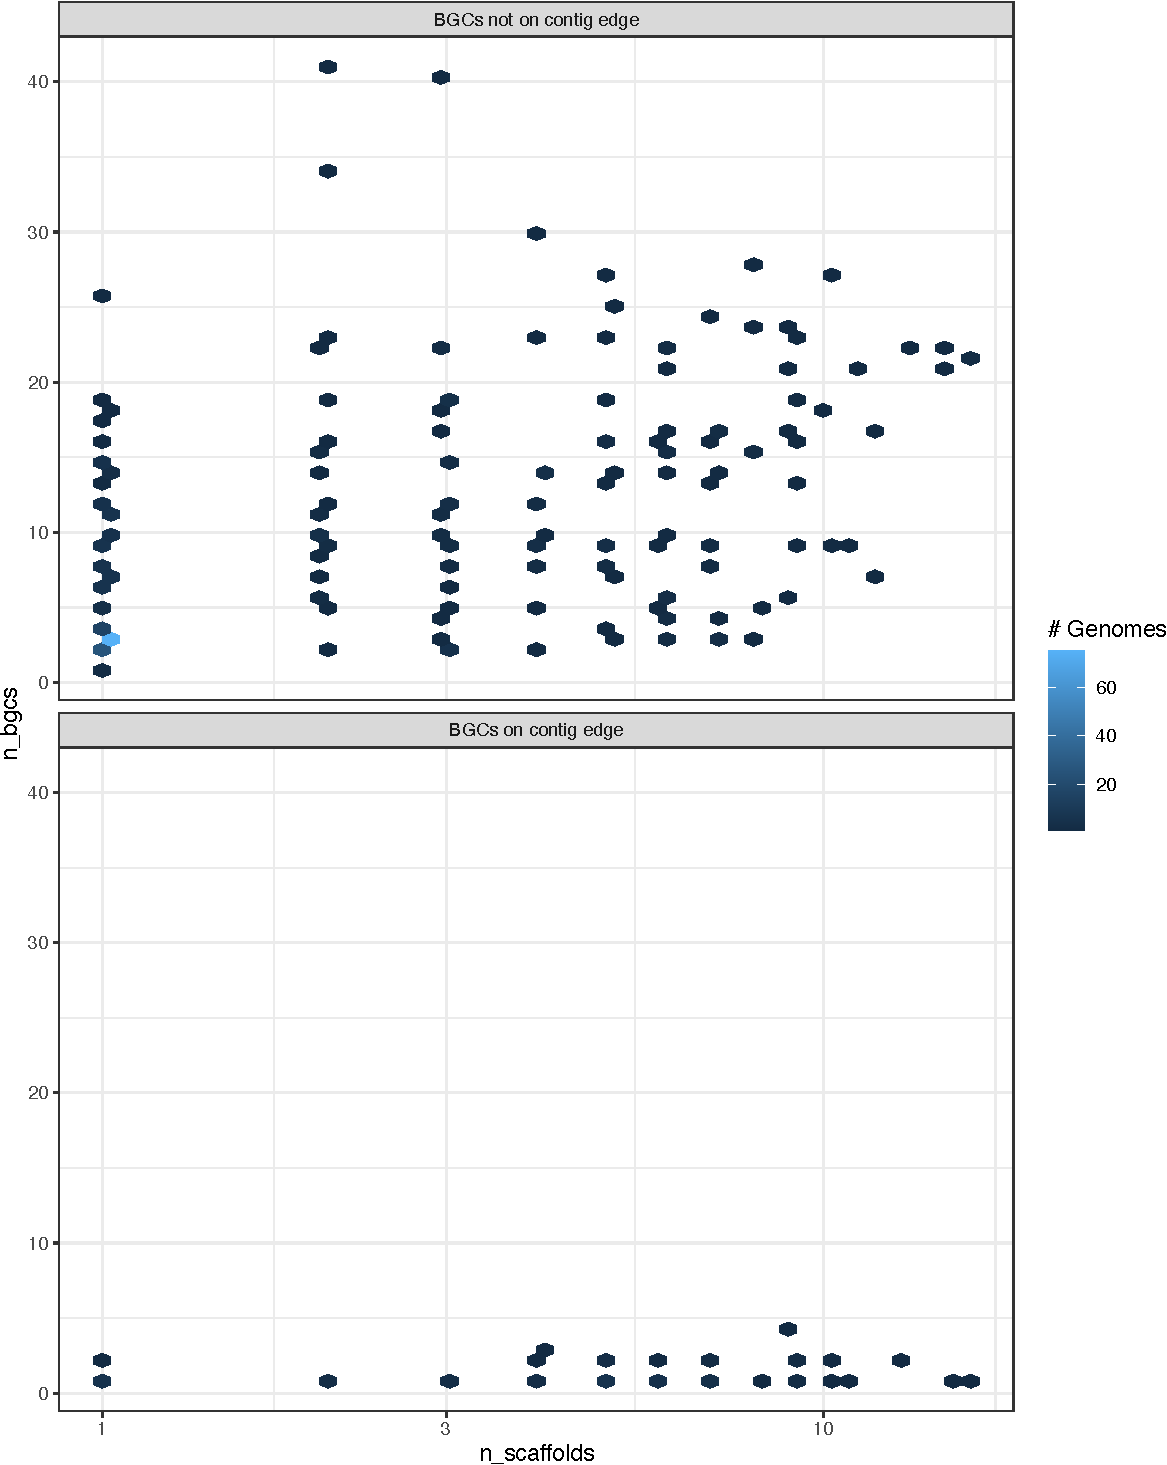
\includegraphics{analysis_files/figure-latex/unnamed-chunk-5-1.pdf}

\hypertarget{analyze-data}{%
\section{Analyze data}\label{analyze-data}}

Now we will proceed with our analysis, with the goal of looking at the
BGC content of phylum Cyanobacteriota across the axes of length, BGC
category, and taxonomy.

Note: AntiSMASH-annotated BGCs are assigned one or more of several dozen
BGC ``classes'' based on the detection rule(s) triggered. These classes
can also be grouped into one of 7 ``categories'' as defined by MIBiG --
namely \texttt{Polyketide}, \texttt{NRP}, \texttt{RiPP},
\texttt{Terpene}, \texttt{Saccharide}, \texttt{Alkaloid}, and
\texttt{Other}.

\hypertarget{summary-statistics-of-bgc-length-across-bgc-categories}{%
\subsubsection{Summary statistics of BGC length across BGC
categories}\label{summary-statistics-of-bgc-length-across-bgc-categories}}

\begin{verbatim}
## # A tibble: 22 x 7
## # Groups:   cats_str [22]
##    cats_str                   n min_len max_len mean_len median_len     sd
##    <fct>                  <int>   <dbl>   <dbl>    <dbl>      <dbl>  <dbl>
##  1 Terpene                  834   13541   39454   20403.     20612.  2079.
##  2 RiPP                     739    7553   76778   29623.     24133  10016.
##  3 NRP                      500   20873   97395   47693.     43942. 10078.
##  4 Polyketide               307   22218   87362   46966.     46241   6996.
##  5 NRP, Polyketide          296   15761  190414   73530.     70899  24984.
##  6 Other                     97   10034   60591   23411.     20762  10296.
##  7 NRP, RiPP                 46   44214  131611   68485.     64902. 19801.
##  8 NRP, Other                32   43141   99576   76136.     78536. 20579.
##  9 NRP, Polyketide, RiPP     21   58186  257631  124101.     91425  63076.
## 10 NRP, Other, Polyketide    18   47242  154012   80890.     73720. 33500.
## # i 12 more rows
\end{verbatim}

\hypertarget{how-many-bgcs-in-each-category-counting-hybrids-of-categories-as-separate}{%
\subsubsection{How many BGCs in each category? (counting hybrids of
categories as
separate)}\label{how-many-bgcs-in-each-category-counting-hybrids-of-categories-as-separate}}

\begin{Shaded}
\begin{Highlighting}[]
\NormalTok{category\_counts }\OtherTok{\textless{}{-}}\NormalTok{ region\_summary }\SpecialCharTok{\%\textgreater{}\%}
  \FunctionTok{ggplot}\NormalTok{(}\FunctionTok{aes}\NormalTok{(}\AttributeTok{y =} \FunctionTok{reorder}\NormalTok{(cats\_str, }\FunctionTok{desc}\NormalTok{(n)))) }\SpecialCharTok{+}
  \FunctionTok{geom\_col}\NormalTok{(}\FunctionTok{aes}\NormalTok{(}\AttributeTok{x =}\NormalTok{ n)) }\SpecialCharTok{+}
  \FunctionTok{scale\_x\_continuous}\NormalTok{(}\AttributeTok{name =} \StringTok{"BGC count"}\NormalTok{, }\AttributeTok{breaks =} \FunctionTok{breaks\_width}\NormalTok{(}\DecValTok{100}\NormalTok{)) }\SpecialCharTok{+}
  \FunctionTok{scale\_y\_discrete}\NormalTok{(}\AttributeTok{name =} \StringTok{"BGC Category"}\NormalTok{) }\SpecialCharTok{+}
  \FunctionTok{theme\_bw}\NormalTok{() }\SpecialCharTok{+}
  \FunctionTok{ggtitle}\NormalTok{(}\StringTok{"Number of BGCs in dataset, divided by category"}\NormalTok{)}
\NormalTok{category\_counts}
\end{Highlighting}
\end{Shaded}

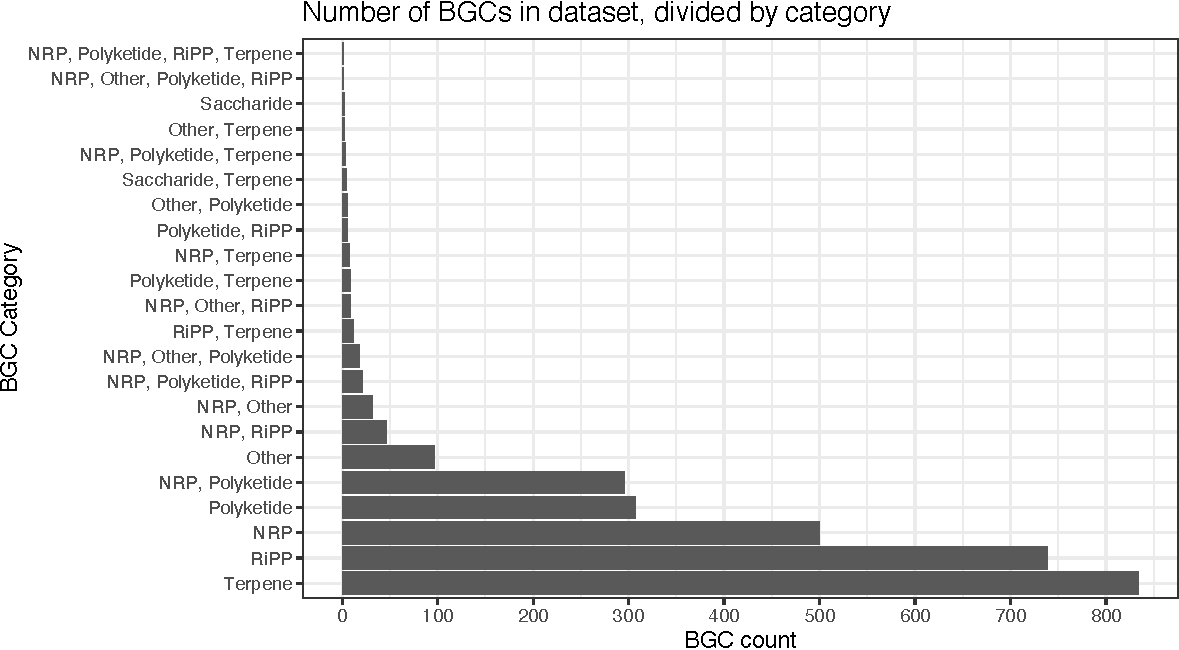
\includegraphics{analysis_files/figure-latex/unnamed-chunk-7-1.pdf}

\begin{Shaded}
\begin{Highlighting}[]
\FunctionTok{ggsave}\NormalTok{(}\StringTok{"./figs/svg/category\_counts.svg"}\NormalTok{, category\_counts, }\AttributeTok{device =} \StringTok{"svg"}\NormalTok{)}
\FunctionTok{ggsave}\NormalTok{(}\StringTok{"./figs/png/category\_counts.png"}\NormalTok{, category\_counts, }\AttributeTok{device =} \StringTok{"png"}\NormalTok{)}
\end{Highlighting}
\end{Shaded}

\hypertarget{how-many-bgcs-in-each-category-lumping-all-hybrids-into-one-except-nrps-pks}{%
\subsubsection{How many BGCs in each category? (lumping all hybrids into
one except
NRPS-PKS)}\label{how-many-bgcs-in-each-category-lumping-all-hybrids-into-one-except-nrps-pks}}

\begin{Shaded}
\begin{Highlighting}[]
\CommentTok{\# Lump any hybrid category with fewer than 80 BGCs into an "all other" category}
\CommentTok{\# {-} Threshold determined arbitrarily to improve visualization}
\NormalTok{region\_summary\_lumped }\OtherTok{\textless{}{-}}\NormalTok{ region\_summary }\SpecialCharTok{\%\textgreater{}\%}
  \FunctionTok{mutate}\NormalTok{(}
    \AttributeTok{group =} \FunctionTok{if\_else}\NormalTok{(n }\SpecialCharTok{\textless{}} \DecValTok{80}\NormalTok{, }\StringTok{"All other hybrids"}\NormalTok{, cats\_str),}
    \AttributeTok{group =}\NormalTok{ group }\SpecialCharTok{\%\textgreater{}\%} \FunctionTok{fct\_reorder}\NormalTok{(n)}
\NormalTok{  )}

\CommentTok{\# Keep a reference DF handy for which categories got lumped}
\NormalTok{lump\_groups }\OtherTok{\textless{}{-}}\NormalTok{ region\_summary\_lumped }\SpecialCharTok{\%\textgreater{}\%} \FunctionTok{select}\NormalTok{(cats\_str, group)}

\CommentTok{\# Use the MIBiG / antiSMASH coloring scheme}
\NormalTok{cat\_colors }\OtherTok{\textless{}{-}} \FunctionTok{c}\NormalTok{(}
  \StringTok{"Polyketide"} \OtherTok{=} \StringTok{"\#f4a460"}\NormalTok{,}
  \StringTok{"NRP"} \OtherTok{=} \StringTok{"\#2e8b57"}\NormalTok{,}
  \StringTok{"RiPP"} \OtherTok{=} \StringTok{"\#4169e1"}\NormalTok{,}
  \StringTok{"Terpene"} \OtherTok{=} \StringTok{"purple"}\NormalTok{,}
  \StringTok{"Saccharide"} \OtherTok{=} \StringTok{"\#deb887"}\NormalTok{,}
  \StringTok{"Other"} \OtherTok{=} \StringTok{"\#191970"}\NormalTok{,}
  \StringTok{"NRP, Polyketide"} \OtherTok{=} \StringTok{"lightsteelblue"}\NormalTok{,}
  \StringTok{"All other hybrids"} \OtherTok{=} \StringTok{"gray50"}
\NormalTok{)}

\CommentTok{\# Plot it}
\NormalTok{lumped\_category\_counts }\OtherTok{\textless{}{-}}\NormalTok{ region\_summary\_lumped }\SpecialCharTok{\%\textgreater{}\%}
  \FunctionTok{ggplot}\NormalTok{(}\FunctionTok{aes}\NormalTok{(}\AttributeTok{y =} \FunctionTok{reorder}\NormalTok{(group, n))) }\SpecialCharTok{+}
  \FunctionTok{geom\_col}\NormalTok{(}\FunctionTok{aes}\NormalTok{(}\AttributeTok{x =}\NormalTok{ n, }\AttributeTok{fill =}\NormalTok{ group)) }\SpecialCharTok{+}
  \FunctionTok{scale\_x\_continuous}\NormalTok{(}\AttributeTok{name =} \StringTok{"BGC count"}\NormalTok{, }\AttributeTok{breaks =} \FunctionTok{breaks\_extended}\NormalTok{()) }\SpecialCharTok{+}
  \FunctionTok{scale\_y\_discrete}\NormalTok{(}\AttributeTok{name =} \StringTok{"BGC Category"}\NormalTok{) }\SpecialCharTok{+}
  \FunctionTok{scale\_fill\_manual}\NormalTok{(}\AttributeTok{values =}\NormalTok{ cat\_colors) }\SpecialCharTok{+}
  \FunctionTok{theme\_bw}\NormalTok{() }\SpecialCharTok{+}
  \FunctionTok{guides}\NormalTok{(}\AttributeTok{fill =} \StringTok{"none"}\NormalTok{)}
\NormalTok{lumped\_category\_counts}
\end{Highlighting}
\end{Shaded}

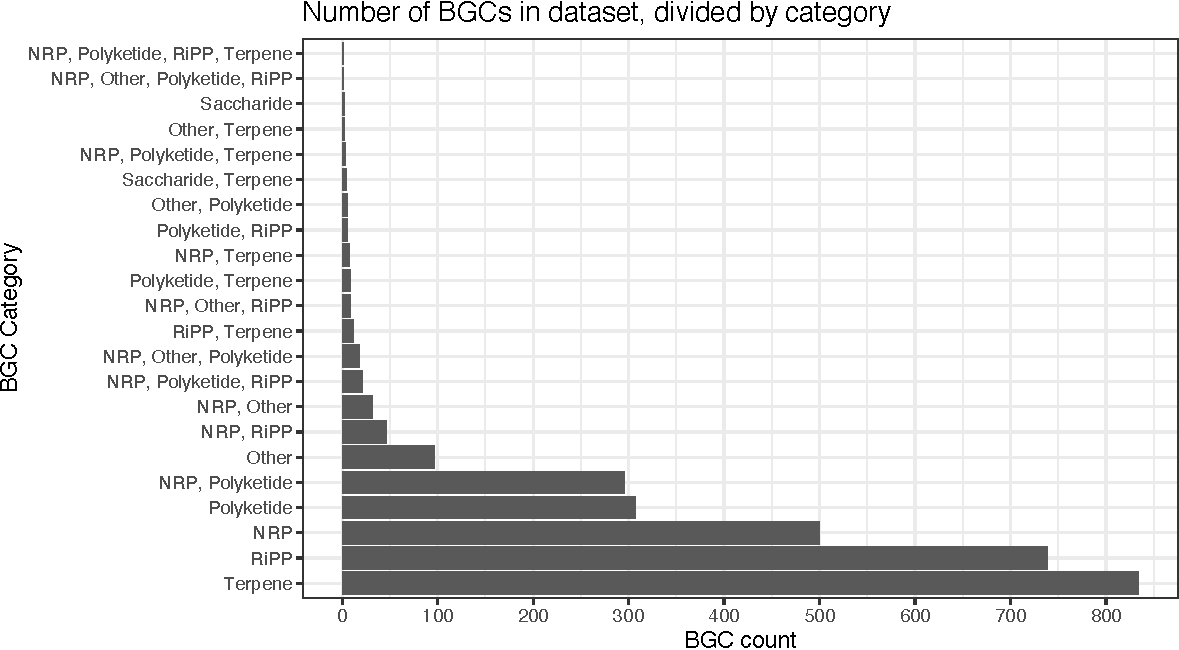
\includegraphics{analysis_files/figure-latex/unnamed-chunk-8-1.pdf}

\begin{Shaded}
\begin{Highlighting}[]
\FunctionTok{ggsave}\NormalTok{(}\StringTok{"./figs/svg/category\_counts\_lumped.svg"}\NormalTok{, lumped\_category\_counts, }\AttributeTok{device =} \StringTok{"svg"}\NormalTok{)}
\FunctionTok{ggsave}\NormalTok{(}\StringTok{"./figs/png/category\_counts\_lumped.png"}\NormalTok{, lumped\_category\_counts, }\AttributeTok{device =} \StringTok{"png"}\NormalTok{)}
\end{Highlighting}
\end{Shaded}

\hypertarget{how-do-bgcs-vary-in-length-by-category-or-combination-of-categories}{%
\subsubsection{How do BGCs vary in length by category (or combination of
categories)?}\label{how-do-bgcs-vary-in-length-by-category-or-combination-of-categories}}

Un-lumped categories

\begin{Shaded}
\begin{Highlighting}[]
\NormalTok{regions\_lumped }\OtherTok{\textless{}{-}}\NormalTok{ regions }\SpecialCharTok{\%\textgreater{}\%} \FunctionTok{left\_join}\NormalTok{(lump\_groups, }\AttributeTok{by =} \StringTok{"cats\_str"}\NormalTok{)}

\NormalTok{region\_hist }\OtherTok{\textless{}{-}} \FunctionTok{ggplot}\NormalTok{(regions\_lumped, }\FunctionTok{aes}\NormalTok{(}
  \AttributeTok{x =}\NormalTok{ region\_length }\SpecialCharTok{/} \DecValTok{1000}\NormalTok{,}
\NormalTok{)) }\SpecialCharTok{+}
  \FunctionTok{geom\_histogram}\NormalTok{(}\FunctionTok{aes}\NormalTok{(}\AttributeTok{fill =}\NormalTok{ group), }\AttributeTok{bins =} \DecValTok{50}\NormalTok{) }\SpecialCharTok{+}
  \FunctionTok{scale\_x\_log10}\NormalTok{(}\AttributeTok{name =} \StringTok{"BGC length (kb)"}\NormalTok{, }\AttributeTok{guide =} \StringTok{"axis\_logticks"}\NormalTok{, }\AttributeTok{breaks =} \FunctionTok{breaks\_log}\NormalTok{(), }\AttributeTok{labels =} \FunctionTok{label\_comma}\NormalTok{()) }\SpecialCharTok{+}
  \FunctionTok{scale\_y\_continuous}\NormalTok{(}\AttributeTok{name =} \StringTok{"BGC count"}\NormalTok{, }\AttributeTok{breaks =} \FunctionTok{breaks\_extended}\NormalTok{(), }\AttributeTok{labels =} \FunctionTok{label\_comma}\NormalTok{()) }\SpecialCharTok{+}
  \FunctionTok{scale\_fill\_manual}\NormalTok{(}\AttributeTok{values =}\NormalTok{ cat\_colors) }\SpecialCharTok{+}
  \FunctionTok{facet\_grid}\NormalTok{(}\AttributeTok{rows =} \FunctionTok{vars}\NormalTok{(cats\_str), }\AttributeTok{scales =} \StringTok{"free\_y"}\NormalTok{) }\SpecialCharTok{+}
  \FunctionTok{theme\_bw}\NormalTok{() }\SpecialCharTok{+}
  \FunctionTok{theme}\NormalTok{(}\AttributeTok{strip.text.y.right =} \FunctionTok{element\_text}\NormalTok{(}\AttributeTok{angle =} \DecValTok{0}\NormalTok{)) }\SpecialCharTok{+}
  \FunctionTok{guides}\NormalTok{(}\AttributeTok{fill =} \ConstantTok{FALSE}\NormalTok{)}

\NormalTok{region\_hist}
\end{Highlighting}
\end{Shaded}

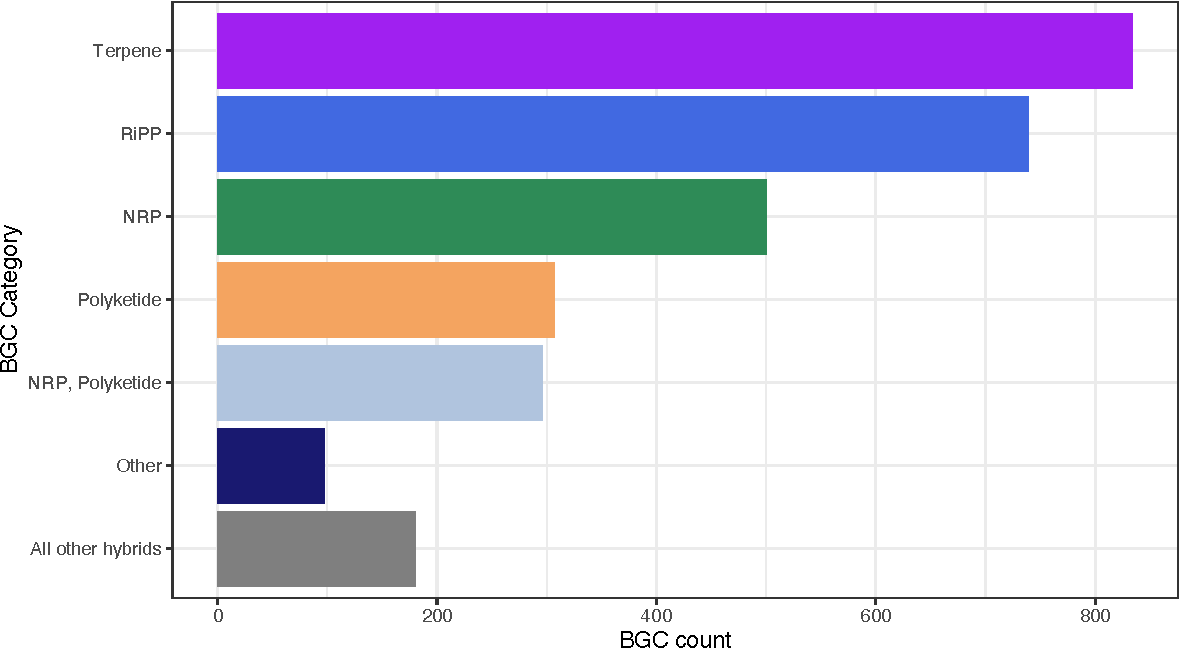
\includegraphics{analysis_files/figure-latex/unnamed-chunk-9-1.pdf}

\begin{Shaded}
\begin{Highlighting}[]
\FunctionTok{ggsave}\NormalTok{(}\StringTok{"./figs/svg/region\_hist.svg"}\NormalTok{, region\_hist, }\AttributeTok{device =} \StringTok{"svg"}\NormalTok{)}
\FunctionTok{ggsave}\NormalTok{(}\StringTok{"./figs/png/region\_hist.png"}\NormalTok{, region\_hist, }\AttributeTok{device =} \StringTok{"png"}\NormalTok{)}
\end{Highlighting}
\end{Shaded}

Lumped categories (again, except for NRPS-PKS hybrids)

\begin{Shaded}
\begin{Highlighting}[]
\NormalTok{region\_hist\_lumped }\OtherTok{\textless{}{-}}\NormalTok{ regions\_lumped }\SpecialCharTok{\%\textgreater{}\%}
  \FunctionTok{filter}\NormalTok{(group }\SpecialCharTok{!=} \StringTok{"All other hybrids"}\NormalTok{) }\SpecialCharTok{\%\textgreater{}\%}
  \FunctionTok{ggplot}\NormalTok{(}\FunctionTok{aes}\NormalTok{(}\AttributeTok{x =}\NormalTok{ region\_length }\SpecialCharTok{/} \DecValTok{1000}\NormalTok{)) }\SpecialCharTok{+}
  \FunctionTok{geom\_histogram}\NormalTok{(}\FunctionTok{aes}\NormalTok{(}\AttributeTok{fill =}\NormalTok{ group), }\AttributeTok{bins =} \DecValTok{50}\NormalTok{) }\SpecialCharTok{+}
  \FunctionTok{scale\_x\_log10}\NormalTok{(}\AttributeTok{name =} \StringTok{"BGC length (kb)"}\NormalTok{, }\AttributeTok{guide =} \StringTok{"axis\_logticks"}\NormalTok{, }\AttributeTok{limits =} \FunctionTok{c}\NormalTok{(}\DecValTok{1}\NormalTok{, }\ConstantTok{NA}\NormalTok{), }\AttributeTok{breaks =} \FunctionTok{c}\NormalTok{(}\DecValTok{1}\NormalTok{, }\DecValTok{5}\NormalTok{, }\DecValTok{10}\NormalTok{, }\DecValTok{50}\NormalTok{, }\DecValTok{100}\NormalTok{, }\DecValTok{200}\NormalTok{)) }\SpecialCharTok{+}
  \FunctionTok{scale\_y\_continuous}\NormalTok{(}\AttributeTok{name =} \StringTok{"BGC count"}\NormalTok{, }\AttributeTok{breaks =} \FunctionTok{breaks\_extended}\NormalTok{(}\AttributeTok{n =} \DecValTok{3}\NormalTok{)) }\SpecialCharTok{+}
  \FunctionTok{scale\_fill\_manual}\NormalTok{(}\AttributeTok{values =}\NormalTok{ cat\_colors) }\SpecialCharTok{+}
  \FunctionTok{facet\_wrap}\NormalTok{(}\FunctionTok{vars}\NormalTok{(group), }\AttributeTok{ncol =} \DecValTok{1}\NormalTok{, }\AttributeTok{scales =} \StringTok{"free\_y"}\NormalTok{) }\SpecialCharTok{+}
  \FunctionTok{guides}\NormalTok{(}\AttributeTok{fill =} \FunctionTok{guide\_legend}\NormalTok{(}\AttributeTok{title =} \StringTok{"BGC Category"}\NormalTok{)) }\SpecialCharTok{+}
  \FunctionTok{theme\_bw}\NormalTok{() }\SpecialCharTok{+}
  \FunctionTok{theme}\NormalTok{(}
    \AttributeTok{strip.background =} \FunctionTok{element\_blank}\NormalTok{(),}
    \AttributeTok{strip.text =} \FunctionTok{element\_blank}\NormalTok{()}
\NormalTok{  )}
\NormalTok{region\_hist\_lumped}
\end{Highlighting}
\end{Shaded}

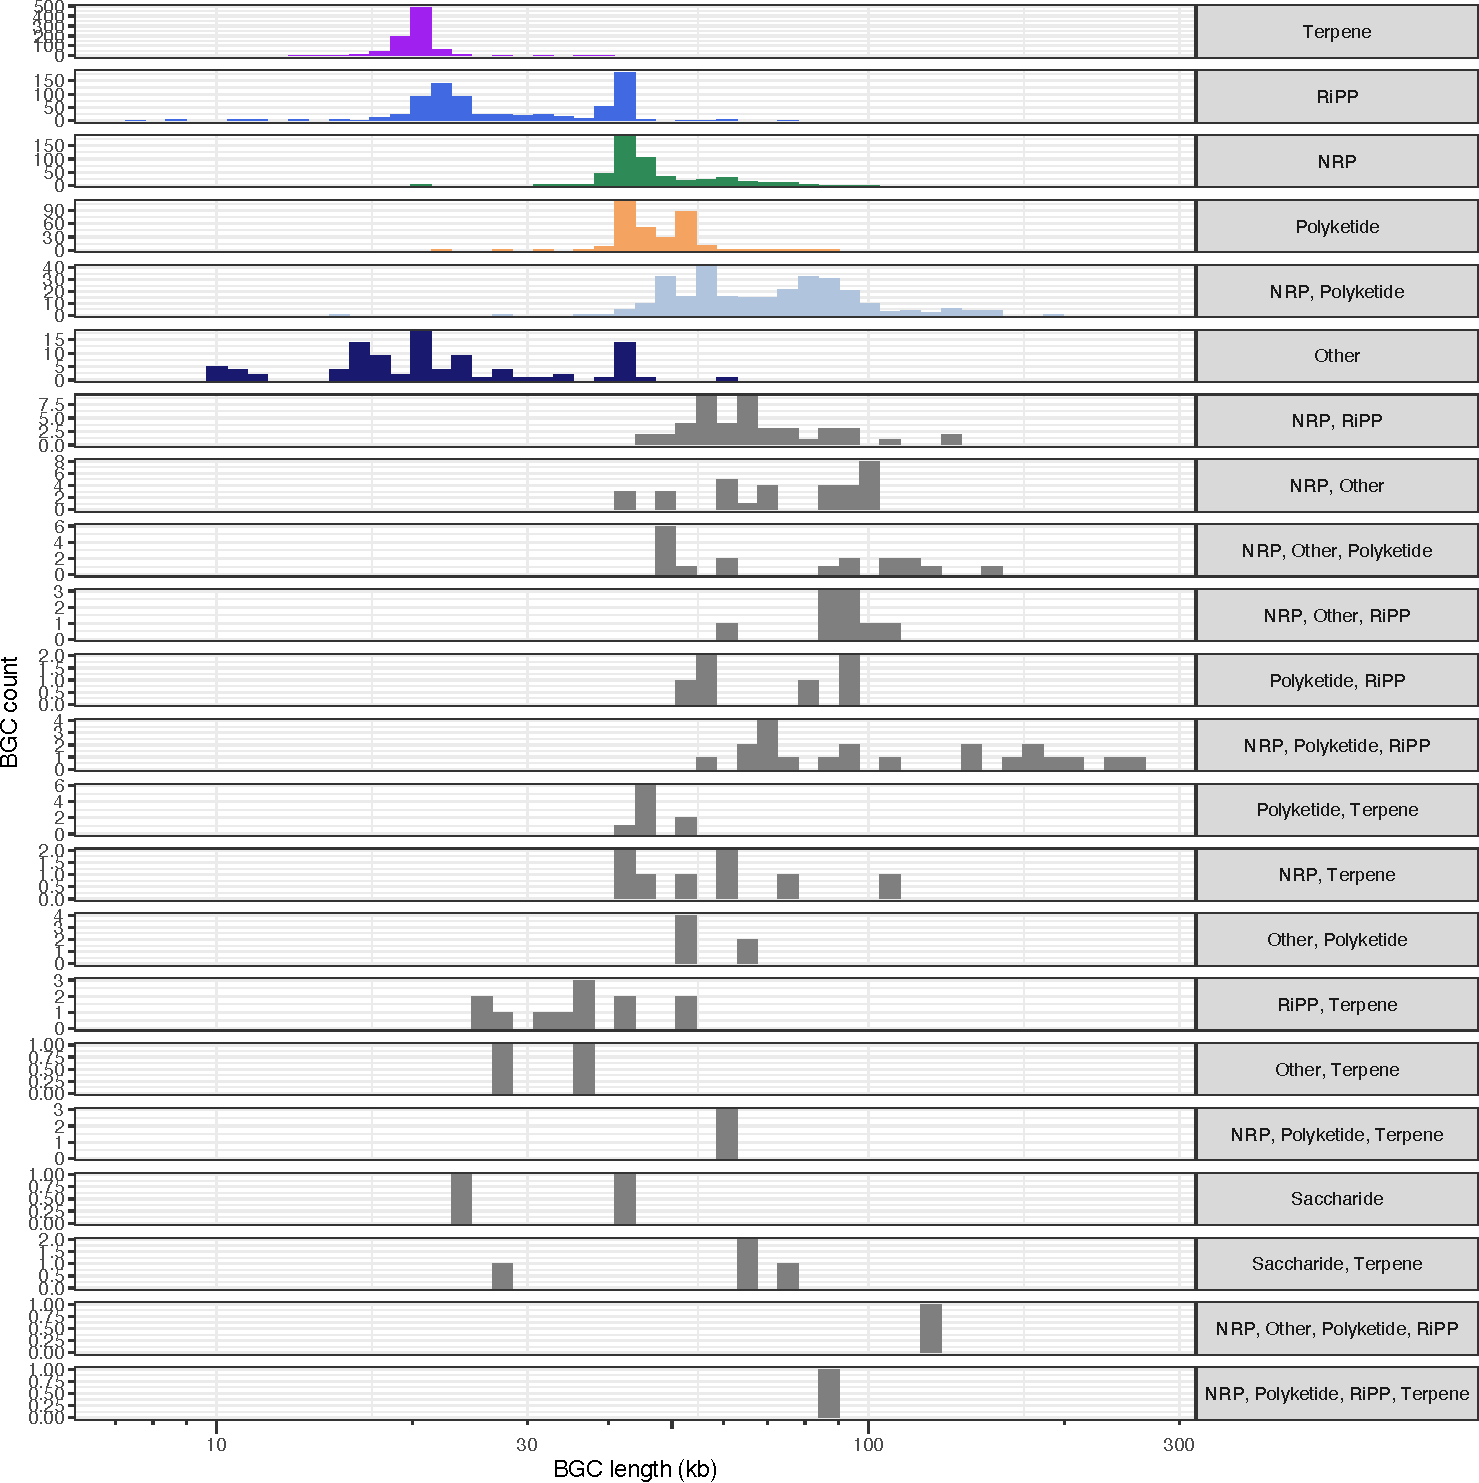
\includegraphics{analysis_files/figure-latex/unnamed-chunk-10-1.pdf}

\begin{Shaded}
\begin{Highlighting}[]
\FunctionTok{ggsave}\NormalTok{(}\StringTok{"./figs/svg/region\_hist\_lumped.svg"}\NormalTok{, region\_hist\_lumped, }\AttributeTok{device =} \StringTok{"svg"}\NormalTok{)}
\FunctionTok{ggsave}\NormalTok{(}\StringTok{"./figs/png/region\_hist\_lumped.png"}\NormalTok{, region\_hist\_lumped, }\AttributeTok{device =} \StringTok{"png"}\NormalTok{)}
\end{Highlighting}
\end{Shaded}

\hypertarget{how-does-bgc-count-vary-across-genera-and-by-category}{%
\subsubsection{How does BGC count vary across genera and by
category?}\label{how-does-bgc-count-vary-across-genera-and-by-category}}

Table:

\begin{Shaded}
\begin{Highlighting}[]
\NormalTok{tax\_count }\OtherTok{\textless{}{-}}\NormalTok{ regions\_lumped }\SpecialCharTok{\%\textgreater{}\%}
  \FunctionTok{group\_by}\NormalTok{(tax\_genus, cats\_str) }\SpecialCharTok{\%\textgreater{}\%}
  \FunctionTok{summarize}\NormalTok{(}\AttributeTok{num\_bgcs =} \FunctionTok{n}\NormalTok{()) }\SpecialCharTok{\%\textgreater{}\%}
  \FunctionTok{mutate}\NormalTok{(}\AttributeTok{tax\_genus =}\NormalTok{ tax\_genus }\SpecialCharTok{\%\textgreater{}\%} \FunctionTok{fct\_reorder}\NormalTok{(num\_bgcs)) }\SpecialCharTok{\%\textgreater{}\%}
  \FunctionTok{left\_join}\NormalTok{(lump\_groups, }\AttributeTok{by =} \StringTok{"cats\_str"}\NormalTok{) }\CommentTok{\# \%\textgreater{}\%}

\NormalTok{tax\_count}
\end{Highlighting}
\end{Shaded}

\begin{verbatim}
## # A tibble: 388 x 4
## # Groups:   tax_genus [70]
##    tax_genus     cats_str        num_bgcs group          
##    <fct>         <fct>              <int> <fct>          
##  1 Acaryochloris Terpene               16 Terpene        
##  2 Acaryochloris RiPP                  12 RiPP           
##  3 Acaryochloris NRP                    2 NRP            
##  4 Acaryochloris Polyketide             2 Polyketide     
##  5 Acaryochloris NRP, Polyketide        2 NRP, Polyketide
##  6 Acaryochloris Other                  4 Other          
##  7 Allocoleopsis Terpene                2 Terpene        
##  8 Allocoleopsis RiPP                   4 RiPP           
##  9 Allocoleopsis NRP                    2 NRP            
## 10 Allocoleopsis NRP, Polyketide        1 NRP, Polyketide
## # i 378 more rows
\end{verbatim}

Raw BGC counts by genus

\begin{Shaded}
\begin{Highlighting}[]
\NormalTok{p\_all }\OtherTok{\textless{}{-}}\NormalTok{ tax\_count }\SpecialCharTok{\%\textgreater{}\%}
  \FunctionTok{group\_by}\NormalTok{(tax\_genus) }\SpecialCharTok{\%\textgreater{}\%}
  \FunctionTok{filter}\NormalTok{(}\FunctionTok{sum}\NormalTok{(num\_bgcs) }\SpecialCharTok{\textgreater{}} \DecValTok{0}\NormalTok{) }\SpecialCharTok{\%\textgreater{}\%}
  \FunctionTok{ggplot}\NormalTok{(}\FunctionTok{aes}\NormalTok{(}\AttributeTok{x =} \FunctionTok{fct\_infreq}\NormalTok{(tax\_genus, }\AttributeTok{w =}\NormalTok{ num\_bgcs))) }\SpecialCharTok{+}
  \FunctionTok{geom\_col}\NormalTok{(}\FunctionTok{aes}\NormalTok{(}\AttributeTok{y =}\NormalTok{ num\_bgcs, }\AttributeTok{fill =}\NormalTok{ group), }\AttributeTok{position =} \FunctionTok{position\_stack}\NormalTok{(}\AttributeTok{reverse =} \ConstantTok{TRUE}\NormalTok{)) }\SpecialCharTok{+}
  \FunctionTok{scale\_y\_continuous}\NormalTok{(}\AttributeTok{name =} \StringTok{"BGC count"}\NormalTok{, }\AttributeTok{breaks =} \FunctionTok{breaks\_extended}\NormalTok{()) }\SpecialCharTok{+}
  \FunctionTok{scale\_x\_discrete}\NormalTok{(}\AttributeTok{name =} \StringTok{"Genus"}\NormalTok{) }\SpecialCharTok{+}
  \FunctionTok{scale\_fill\_manual}\NormalTok{(}\AttributeTok{name =} \StringTok{"BGC Category"}\NormalTok{, }\AttributeTok{values =}\NormalTok{ cat\_colors) }\SpecialCharTok{+}
  \FunctionTok{coord\_flip}\NormalTok{() }\SpecialCharTok{+}
  \FunctionTok{theme\_bw}\NormalTok{() }\SpecialCharTok{+}
  \FunctionTok{ggtitle}\NormalTok{(}\StringTok{"(all genera)"}\NormalTok{)}
\NormalTok{p\_all}
\end{Highlighting}
\end{Shaded}

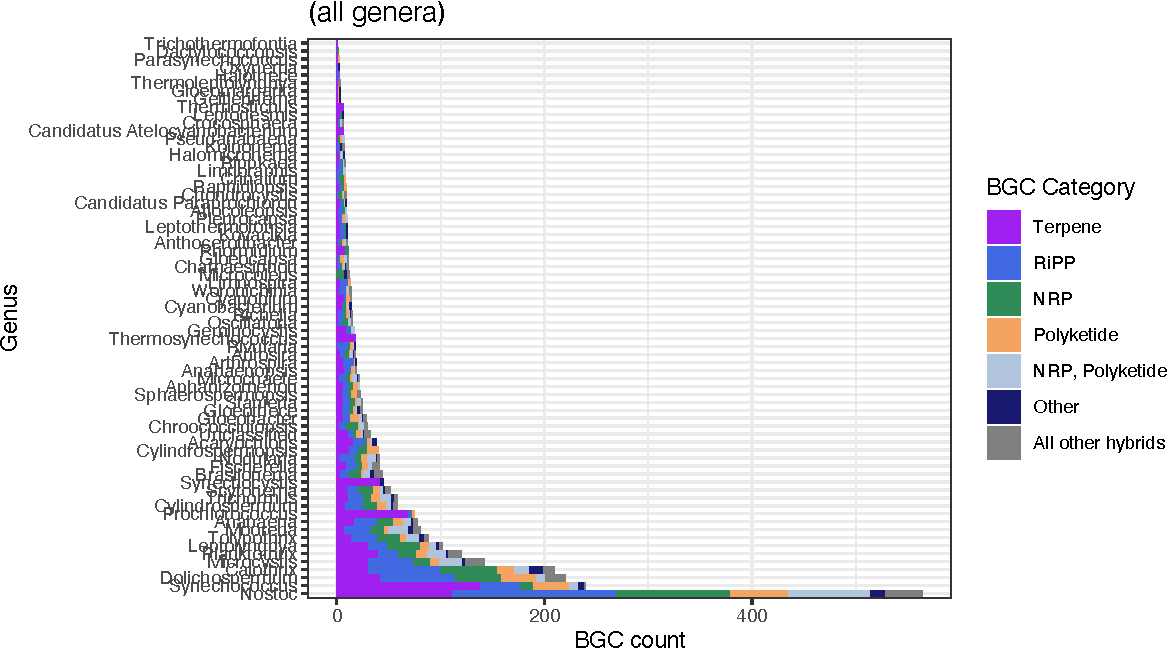
\includegraphics{analysis_files/figure-latex/unnamed-chunk-12-1.pdf}

\begin{Shaded}
\begin{Highlighting}[]
\FunctionTok{ggsave}\NormalTok{(}\StringTok{"./figs/svg/genus\_counts\_all.svg"}\NormalTok{, p\_all, }\AttributeTok{device =} \StringTok{"svg"}\NormalTok{)}
\FunctionTok{ggsave}\NormalTok{(}\StringTok{"./figs/png/genus\_counts\_all.png"}\NormalTok{, p\_all, }\AttributeTok{device =} \StringTok{"png"}\NormalTok{)}
\end{Highlighting}
\end{Shaded}

In order to normalize BGC counts to a per-genome basis, we must also
know how many Cyano genomes \emph{lacked} BGCs (as detected by
antiSMASH).

\begin{Shaded}
\begin{Highlighting}[]
\CommentTok{\# Plaintext file listing all the accessions that had no BGCs}
\NormalTok{cyano\_nohits }\OtherTok{\textless{}{-}} \FunctionTok{read\_tsv}\NormalTok{(}\StringTok{"data/ncbi\_cyano\_nohit\_accs.txt"}\NormalTok{, }\AttributeTok{col\_names =} \FunctionTok{c}\NormalTok{(}\StringTok{"accession\_id"}\NormalTok{)) }\SpecialCharTok{\%\textgreater{}\%}
  \FunctionTok{left\_join}\NormalTok{(cyano\_asm\_tax, }\AttributeTok{by =} \FunctionTok{join\_by}\NormalTok{(accession\_id }\SpecialCharTok{==}\NormalTok{ assembly\_accession))}

\CommentTok{\# Incorporate these into our genome counts}
\NormalTok{cyano\_nohit\_genus\_counts }\OtherTok{\textless{}{-}}\NormalTok{ cyano\_nohits }\SpecialCharTok{\%\textgreater{}\%}
  \FunctionTok{group\_by}\NormalTok{(genus) }\SpecialCharTok{\%\textgreater{}\%}
  \FunctionTok{summarize}\NormalTok{(}\AttributeTok{n\_nohits =} \FunctionTok{n}\NormalTok{()) }\SpecialCharTok{\%\textgreater{}\%}
  \FunctionTok{mutate}\NormalTok{(}\AttributeTok{genus =} \FunctionTok{replace\_na}\NormalTok{(genus, }\StringTok{"Unclassified"}\NormalTok{)) }\SpecialCharTok{\%\textgreater{}\%}
  \FunctionTok{arrange}\NormalTok{(genus)}

\NormalTok{genomes\_by\_genus }\OtherTok{\textless{}{-}} \FunctionTok{read\_tsv}\NormalTok{(}\StringTok{"data/2025{-}02{-}25{-}1442{-}cyano\_smc\_src\_counts\_by\_genus.tsv"}\NormalTok{)}
\NormalTok{genomes\_by\_genus }\OtherTok{\textless{}{-}}\NormalTok{ genomes\_by\_genus }\SpecialCharTok{\%\textgreater{}\%}
  \FunctionTok{left\_join}\NormalTok{(cyano\_nohit\_genus\_counts, }\AttributeTok{by =} \FunctionTok{join\_by}\NormalTok{(tax\_genus }\SpecialCharTok{==}\NormalTok{ genus)) }\SpecialCharTok{\%\textgreater{}\%}
  \FunctionTok{mutate}\NormalTok{(}\AttributeTok{n\_nohits =} \FunctionTok{replace\_na}\NormalTok{(n\_nohits, }\DecValTok{0}\NormalTok{)) }\SpecialCharTok{\%\textgreater{}\%}
  \FunctionTok{mutate}\NormalTok{(}\AttributeTok{tot\_genomes =}\NormalTok{ n\_nohits }\SpecialCharTok{+}\NormalTok{ n\_sources, }\AttributeTok{.keep =} \StringTok{"unused"}\NormalTok{)}
\end{Highlighting}
\end{Shaded}

Plot the BGCs per genome (normalized to 100\%) alongside number of BGCs
per genus and genomes per genus

\begin{Shaded}
\begin{Highlighting}[]
\CommentTok{\# Prepare the dataframe specific to this set of plots}
\NormalTok{df\_plots }\OtherTok{\textless{}{-}}\NormalTok{ tax\_count }\SpecialCharTok{\%\textgreater{}\%}
  \FunctionTok{filter}\NormalTok{(tax\_genus }\SpecialCharTok{!=} \StringTok{"Unclassified"}\NormalTok{) }\SpecialCharTok{\%\textgreater{}\%}
  \FunctionTok{left\_join}\NormalTok{(genomes\_by\_genus, }\AttributeTok{by =} \StringTok{"tax\_genus"}\NormalTok{) }\SpecialCharTok{\%\textgreater{}\%}
  \FunctionTok{mutate}\NormalTok{(}\AttributeTok{bgc\_dens =}\NormalTok{ num\_bgcs }\SpecialCharTok{/}\NormalTok{ tot\_genomes) }\SpecialCharTok{\%\textgreater{}\%}
  \FunctionTok{group\_by}\NormalTok{(tax\_genus) }\SpecialCharTok{\%\textgreater{}\%}
  \FunctionTok{mutate}\NormalTok{(}\AttributeTok{tot\_bgc\_dens =} \FunctionTok{sum}\NormalTok{(bgc\_dens), }\AttributeTok{tot\_bgcs =} \FunctionTok{sum}\NormalTok{(num\_bgcs))}

\CommentTok{\# Plot BGCs per genome, colored by category and divided by genus}
\NormalTok{p\_bgc\_dens }\OtherTok{\textless{}{-}}\NormalTok{ df\_plots }\SpecialCharTok{\%\textgreater{}\%}
  \FunctionTok{ggplot}\NormalTok{(}\FunctionTok{aes}\NormalTok{(}\AttributeTok{x =} \FunctionTok{fct\_rev}\NormalTok{(tax\_genus))) }\SpecialCharTok{+}
  \FunctionTok{geom\_col}\NormalTok{(}\FunctionTok{aes}\NormalTok{(}\AttributeTok{y =}\NormalTok{ bgc\_dens, }\AttributeTok{fill =}\NormalTok{ group), }\AttributeTok{position =} \FunctionTok{position\_fill}\NormalTok{(}\AttributeTok{reverse =} \ConstantTok{TRUE}\NormalTok{)) }\SpecialCharTok{+}
  \FunctionTok{scale\_y\_continuous}\NormalTok{(}\AttributeTok{name =} \StringTok{"BGC proportion"}\NormalTok{) }\SpecialCharTok{+}
  \FunctionTok{scale\_x\_discrete}\NormalTok{(}\AttributeTok{name =} \StringTok{"Genus"}\NormalTok{) }\SpecialCharTok{+}
  \FunctionTok{scale\_fill\_manual}\NormalTok{(}\AttributeTok{name =} \StringTok{"BGC Category"}\NormalTok{, }\AttributeTok{values =}\NormalTok{ cat\_colors) }\SpecialCharTok{+}
  \FunctionTok{coord\_flip}\NormalTok{() }\SpecialCharTok{+}
  \FunctionTok{theme\_bw}\NormalTok{() }\SpecialCharTok{+}
  \FunctionTok{theme}\NormalTok{(}\AttributeTok{legend.position =} \StringTok{"bottom"}\NormalTok{)}
\CommentTok{\# p\_bgc\_dens}

\CommentTok{\# Plot total BGC count by genus}
\NormalTok{p\_bgc\_ct }\OtherTok{\textless{}{-}}\NormalTok{ df\_plots }\SpecialCharTok{\%\textgreater{}\%}
  \FunctionTok{ggplot}\NormalTok{(}\FunctionTok{aes}\NormalTok{(}\AttributeTok{x =} \FunctionTok{fct\_rev}\NormalTok{(tax\_genus))) }\SpecialCharTok{+}
  \FunctionTok{geom\_col}\NormalTok{(}\FunctionTok{aes}\NormalTok{(}\AttributeTok{y =}\NormalTok{ tot\_bgcs), }\AttributeTok{data =}\NormalTok{ df\_plots }\SpecialCharTok{\%\textgreater{}\%} \FunctionTok{select}\NormalTok{(tax\_genus, tot\_bgcs, tot\_bgc\_dens) }\SpecialCharTok{\%\textgreater{}\%} \FunctionTok{distinct}\NormalTok{()) }\SpecialCharTok{+}
  \FunctionTok{scale\_y\_continuous}\NormalTok{(}
    \AttributeTok{name =} \StringTok{"BGC count"}\NormalTok{,}
    \AttributeTok{trans =} \FunctionTok{transform\_pseudo\_log}\NormalTok{(}\AttributeTok{base =} \DecValTok{10}\NormalTok{),}
    \AttributeTok{breaks =} \FunctionTok{c}\NormalTok{(}\DecValTok{0}\NormalTok{, }\DecValTok{1}\NormalTok{, }\DecValTok{5}\NormalTok{, }\DecValTok{10}\NormalTok{, }\DecValTok{20}\NormalTok{, }\DecValTok{50}\NormalTok{, }\DecValTok{100}\NormalTok{, }\DecValTok{200}\NormalTok{, }\DecValTok{500}\NormalTok{)}
\NormalTok{  ) }\SpecialCharTok{+}
  \FunctionTok{coord\_flip}\NormalTok{() }\SpecialCharTok{+}
  \FunctionTok{theme\_bw}\NormalTok{() }\SpecialCharTok{+}
  \FunctionTok{theme}\NormalTok{(}
    \AttributeTok{axis.title.y =} \FunctionTok{element\_blank}\NormalTok{(),}
    \AttributeTok{axis.text.y =} \FunctionTok{element\_blank}\NormalTok{()}
\NormalTok{  )}

\CommentTok{\# Plot genome count by genus}
\NormalTok{genome\_counts }\OtherTok{\textless{}{-}}\NormalTok{ df\_plots }\SpecialCharTok{\%\textgreater{}\%}
  \FunctionTok{group\_by}\NormalTok{(tax\_genus, tot\_genomes) }\SpecialCharTok{\%\textgreater{}\%}
  \FunctionTok{summarize}\NormalTok{(}\AttributeTok{tot\_bgc\_dens =} \FunctionTok{sum}\NormalTok{(bgc\_dens), }\AttributeTok{tot\_bgcs =} \FunctionTok{sum}\NormalTok{(num\_bgcs)) }\SpecialCharTok{\%\textgreater{}\%}
  \FunctionTok{arrange}\NormalTok{(tot\_bgc\_dens)}
\NormalTok{genome\_counts}
\end{Highlighting}
\end{Shaded}

\begin{verbatim}
## # A tibble: 69 x 4
## # Groups:   tax_genus [69]
##    tax_genus       tot_genomes tot_bgc_dens tot_bgcs
##    <chr>                 <dbl>        <dbl>    <int>
##  1 Prochlorococcus        1023       0.0733       75
##  2 Pseudanabaena            75       0.0933        7
##  3 Cyanobium               131       0.107        14
##  4 Microcoleus              66       0.182        12
##  5 Crocosphaera             19       0.316         6
##  6 Phormidium               32       0.344        11
##  7 Synechococcus           579       0.415       240
##  8 Microcystis             329       0.432       142
##  9 Aphanizomenon            38       0.579        22
## 10 Fischerella              64       0.641        41
## # i 59 more rows
\end{verbatim}

\begin{Shaded}
\begin{Highlighting}[]
\NormalTok{p\_genome\_ct }\OtherTok{\textless{}{-}}\NormalTok{ genome\_counts }\SpecialCharTok{\%\textgreater{}\%}
  \FunctionTok{ggplot}\NormalTok{(}\FunctionTok{aes}\NormalTok{(}\AttributeTok{x =} \FunctionTok{fct\_rev}\NormalTok{(tax\_genus))) }\SpecialCharTok{+}
  \FunctionTok{geom\_col}\NormalTok{(}\FunctionTok{aes}\NormalTok{(}\AttributeTok{y =}\NormalTok{ tot\_genomes)) }\SpecialCharTok{+}
  \FunctionTok{scale\_y\_continuous}\NormalTok{(}
    \AttributeTok{name =} \StringTok{"Genome count"}\NormalTok{,}
    \AttributeTok{trans =} \FunctionTok{transform\_pseudo\_log}\NormalTok{(}\AttributeTok{base =} \DecValTok{10}\NormalTok{),}
    \AttributeTok{breaks =} \FunctionTok{c}\NormalTok{(}\DecValTok{0}\NormalTok{, }\DecValTok{1}\NormalTok{, }\DecValTok{5}\NormalTok{, }\DecValTok{10}\NormalTok{, }\DecValTok{20}\NormalTok{, }\DecValTok{50}\NormalTok{, }\DecValTok{100}\NormalTok{, }\DecValTok{200}\NormalTok{, }\DecValTok{500}\NormalTok{, }\DecValTok{1000}\NormalTok{)}
\NormalTok{  ) }\SpecialCharTok{+}
  \FunctionTok{coord\_flip}\NormalTok{() }\SpecialCharTok{+}
  \FunctionTok{theme\_bw}\NormalTok{() }\SpecialCharTok{+}
  \FunctionTok{theme}\NormalTok{(}
    \AttributeTok{axis.title.y =} \FunctionTok{element\_blank}\NormalTok{(),}
    \AttributeTok{axis.text.y =} \FunctionTok{element\_blank}\NormalTok{()}
\NormalTok{  )}
\CommentTok{\# p\_genome\_ct}

\CommentTok{\# Plot them all together}
\NormalTok{p4 }\OtherTok{\textless{}{-}} \FunctionTok{plot\_grid}\NormalTok{(p\_bgc\_dens, p\_bgc\_ct, p\_genome\_ct, }\AttributeTok{align =} \StringTok{"h"}\NormalTok{, }\AttributeTok{rel\_widths =} \FunctionTok{c}\NormalTok{(}\DecValTok{3}\NormalTok{, }\DecValTok{1}\NormalTok{, }\DecValTok{1}\NormalTok{), }\AttributeTok{nrow =} \DecValTok{1}\NormalTok{)}
\NormalTok{p4}
\end{Highlighting}
\end{Shaded}

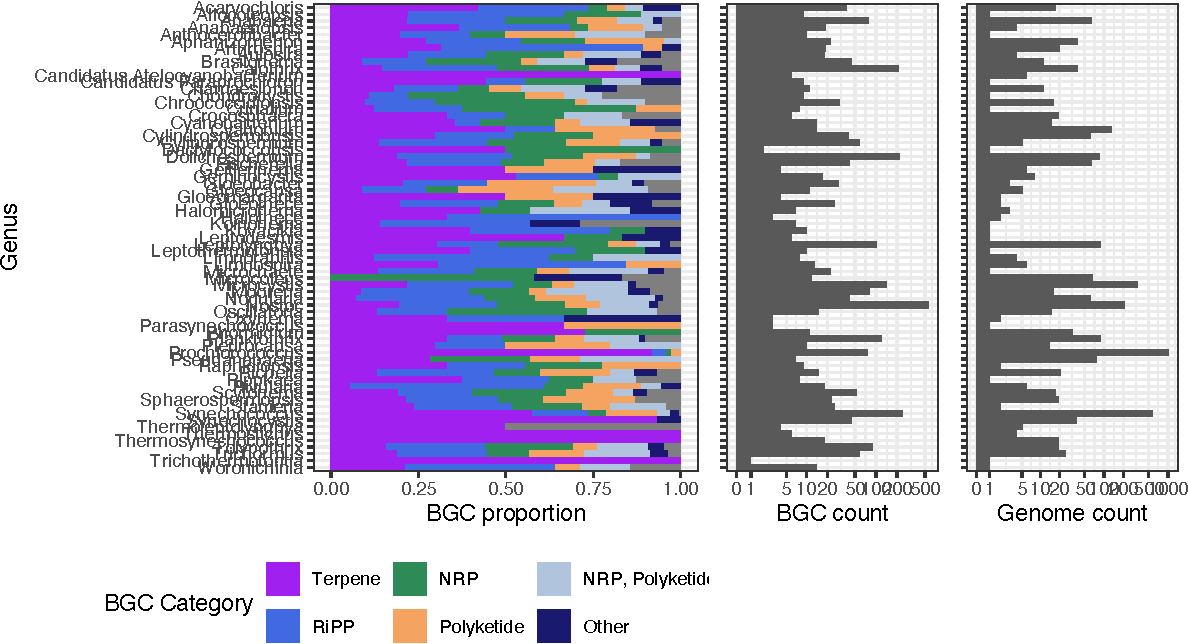
\includegraphics{analysis_files/figure-latex/unnamed-chunk-14-1.pdf}

\begin{Shaded}
\begin{Highlighting}[]
\FunctionTok{ggsave}\NormalTok{(}\StringTok{"./figs/png/split\_proportional.png"}\NormalTok{, p4, }\AttributeTok{width =} \DecValTok{8}\NormalTok{, }\AttributeTok{height =} \DecValTok{11}\NormalTok{, }\AttributeTok{device =} \StringTok{"png"}\NormalTok{)}
\end{Highlighting}
\end{Shaded}

Plot the BGCs per genome (not normalized to 100\%) alongside number of
BGCs per genus and genomes per genus

\begin{Shaded}
\begin{Highlighting}[]
\CommentTok{\# Prepare a dataframe specific to this set of plots}
\CommentTok{\# df\_plots \textless{}{-} tax\_count \%\textgreater{}\%}
\CommentTok{\#   filter(tax\_genus != "Unclassified") \%\textgreater{}\%}
\CommentTok{\#   left\_join(genomes\_by\_genus, by = "tax\_genus") \%\textgreater{}\%}
\CommentTok{\#   mutate(bgc\_dens = num\_bgcs / tot\_genomes) \%\textgreater{}\%}
\CommentTok{\#   group\_by(tax\_genus) \%\textgreater{}\%}
\CommentTok{\#   mutate(tot\_bgc\_dens = sum(bgc\_dens), tot\_bgcs = sum(num\_bgcs))}

\CommentTok{\# Plot BGCs per genome, colored by category and divided by genus}
\NormalTok{p\_bgc\_dens }\OtherTok{\textless{}{-}}\NormalTok{ df\_plots }\SpecialCharTok{\%\textgreater{}\%}
  \FunctionTok{ggplot}\NormalTok{(}\FunctionTok{aes}\NormalTok{(}\AttributeTok{x =} \FunctionTok{fct\_reorder}\NormalTok{(tax\_genus, tot\_bgc\_dens, }\AttributeTok{.desc =}\NormalTok{ T))) }\SpecialCharTok{+}
  \FunctionTok{geom\_col}\NormalTok{(}\FunctionTok{aes}\NormalTok{(}\AttributeTok{y =}\NormalTok{ bgc\_dens, }\AttributeTok{fill =}\NormalTok{ group), }\AttributeTok{position =} \FunctionTok{position\_stack}\NormalTok{(}\AttributeTok{reverse =} \ConstantTok{TRUE}\NormalTok{)) }\SpecialCharTok{+}
  \FunctionTok{scale\_y\_continuous}\NormalTok{(}\AttributeTok{name =} \StringTok{"BGCs per genome"}\NormalTok{) }\SpecialCharTok{+}
  \FunctionTok{scale\_x\_discrete}\NormalTok{(}\AttributeTok{name =} \StringTok{"Genus"}\NormalTok{) }\SpecialCharTok{+}
  \FunctionTok{scale\_fill\_manual}\NormalTok{(}\AttributeTok{name =} \StringTok{"BGC Category"}\NormalTok{, }\AttributeTok{values =}\NormalTok{ cat\_colors) }\SpecialCharTok{+}
  \FunctionTok{coord\_flip}\NormalTok{() }\SpecialCharTok{+}
  \FunctionTok{guides}\NormalTok{(}\AttributeTok{fill =} \FunctionTok{guide\_legend}\NormalTok{(}\AttributeTok{position =} \StringTok{"inside"}\NormalTok{)) }\SpecialCharTok{+}
  \FunctionTok{theme\_bw}\NormalTok{() }\SpecialCharTok{+}
  \FunctionTok{theme}\NormalTok{(}\AttributeTok{legend.justification.inside =} \FunctionTok{c}\NormalTok{(}\FloatTok{0.99}\NormalTok{, }\FloatTok{0.99}\NormalTok{))}
\CommentTok{\# p\_bgc\_dens}

\CommentTok{\# Plot total BGC count by genus}
\NormalTok{p\_bgc\_ct }\OtherTok{\textless{}{-}}\NormalTok{ df\_plots }\SpecialCharTok{\%\textgreater{}\%}
  \FunctionTok{ggplot}\NormalTok{(}\FunctionTok{aes}\NormalTok{(}\AttributeTok{x =} \FunctionTok{fct\_reorder}\NormalTok{(tax\_genus, tot\_bgc\_dens, }\AttributeTok{.desc =}\NormalTok{ T))) }\SpecialCharTok{+}
  \FunctionTok{geom\_col}\NormalTok{(}\FunctionTok{aes}\NormalTok{(}\AttributeTok{y =}\NormalTok{ tot\_bgcs), }\AttributeTok{data =}\NormalTok{ df\_plots }\SpecialCharTok{\%\textgreater{}\%} \FunctionTok{select}\NormalTok{(tax\_genus, tot\_bgcs, tot\_bgc\_dens) }\SpecialCharTok{\%\textgreater{}\%} \FunctionTok{distinct}\NormalTok{()) }\SpecialCharTok{+}
  \FunctionTok{scale\_y\_continuous}\NormalTok{(}
    \AttributeTok{name =} \StringTok{"BGC count"}\NormalTok{,}
    \AttributeTok{trans =} \FunctionTok{transform\_pseudo\_log}\NormalTok{(}\AttributeTok{base =} \DecValTok{10}\NormalTok{),}
    \AttributeTok{breaks =} \FunctionTok{c}\NormalTok{(}\DecValTok{0}\NormalTok{, }\DecValTok{1}\NormalTok{, }\DecValTok{5}\NormalTok{, }\DecValTok{10}\NormalTok{, }\DecValTok{100}\NormalTok{, }\DecValTok{500}\NormalTok{)}
\NormalTok{  ) }\SpecialCharTok{+}
  \FunctionTok{coord\_flip}\NormalTok{() }\SpecialCharTok{+}
  \FunctionTok{theme\_bw}\NormalTok{() }\SpecialCharTok{+}
  \FunctionTok{theme}\NormalTok{(}
    \AttributeTok{axis.title.y =} \FunctionTok{element\_blank}\NormalTok{(),}
    \AttributeTok{axis.text.y =} \FunctionTok{element\_blank}\NormalTok{()}
\NormalTok{  )}

\CommentTok{\# Plot genome count by genus}
\CommentTok{\# genome\_counts \textless{}{-} df\_plots \%\textgreater{}\%}
\CommentTok{\#   group\_by(tax\_genus, tot\_genomes) \%\textgreater{}\%}
\CommentTok{\#   summarize(tot\_bgc\_dens = sum(bgc\_dens), tot\_bgcs = sum(num\_bgcs)) \%\textgreater{}\%}
\CommentTok{\#   arrange(tot\_bgc\_dens)}
\CommentTok{\# genome\_counts}

\NormalTok{p\_genome\_ct }\OtherTok{\textless{}{-}}\NormalTok{ genome\_counts }\SpecialCharTok{\%\textgreater{}\%}
  \FunctionTok{ggplot}\NormalTok{(}\FunctionTok{aes}\NormalTok{(}\AttributeTok{x =} \FunctionTok{fct\_reorder}\NormalTok{(tax\_genus, tot\_bgc\_dens, }\AttributeTok{.desc =}\NormalTok{ T))) }\SpecialCharTok{+}
  \FunctionTok{geom\_col}\NormalTok{(}\FunctionTok{aes}\NormalTok{(}\AttributeTok{y =}\NormalTok{ tot\_genomes)) }\SpecialCharTok{+}
  \FunctionTok{scale\_y\_continuous}\NormalTok{(}\AttributeTok{name =} \StringTok{"Genome count"}\NormalTok{, }\AttributeTok{trans =}\NormalTok{ scales}\SpecialCharTok{::}\FunctionTok{transform\_pseudo\_log}\NormalTok{(}\AttributeTok{base =} \DecValTok{10}\NormalTok{), }\AttributeTok{breaks =} \FunctionTok{c}\NormalTok{(}\DecValTok{0}\NormalTok{, }\DecValTok{1}\NormalTok{, }\DecValTok{5}\NormalTok{, }\DecValTok{10}\NormalTok{, }\DecValTok{100}\NormalTok{, }\DecValTok{1000}\NormalTok{)) }\SpecialCharTok{+}
  \FunctionTok{coord\_flip}\NormalTok{() }\SpecialCharTok{+}
  \FunctionTok{theme\_bw}\NormalTok{() }\SpecialCharTok{+}
  \FunctionTok{theme}\NormalTok{(}
    \AttributeTok{axis.title.y =} \FunctionTok{element\_blank}\NormalTok{(),}
    \AttributeTok{axis.text.y =} \FunctionTok{element\_blank}\NormalTok{()}
\NormalTok{  )}
\CommentTok{\# p\_genome\_ct}

\CommentTok{\# Plot them all together}
\NormalTok{p5 }\OtherTok{\textless{}{-}} \FunctionTok{plot\_grid}\NormalTok{(p\_bgc\_dens, p\_bgc\_ct, p\_genome\_ct, }\AttributeTok{align =} \StringTok{"h"}\NormalTok{, }\AttributeTok{rel\_widths =} \FunctionTok{c}\NormalTok{(}\DecValTok{3}\NormalTok{, }\DecValTok{1}\NormalTok{, }\DecValTok{1}\NormalTok{), }\AttributeTok{nrow =} \DecValTok{1}\NormalTok{)}
\NormalTok{df\_plots}
\end{Highlighting}
\end{Shaded}

\begin{verbatim}
## # A tibble: 378 x 8
## # Groups:   tax_genus [69]
##    tax_genus  cats_str num_bgcs group tot_genomes bgc_dens tot_bgc_dens tot_bgcs
##    <chr>      <fct>       <int> <fct>       <dbl>    <dbl>        <dbl>    <int>
##  1 Acaryochl~ Terpene        16 Terp~          17    0.941         2.24       38
##  2 Acaryochl~ RiPP           12 RiPP           17    0.706         2.24       38
##  3 Acaryochl~ NRP             2 NRP            17    0.118         2.24       38
##  4 Acaryochl~ Polyket~        2 Poly~          17    0.118         2.24       38
##  5 Acaryochl~ NRP, Po~        2 NRP,~          17    0.118         2.24       38
##  6 Acaryochl~ Other           4 Other          17    0.235         2.24       38
##  7 Allocoleo~ Terpene         2 Terp~           1    2             9           9
##  8 Allocoleo~ RiPP            4 RiPP            1    4             9           9
##  9 Allocoleo~ NRP             2 NRP             1    2             9           9
## 10 Allocoleo~ NRP, Po~        1 NRP,~           1    1             9           9
## # i 368 more rows
\end{verbatim}

\begin{Shaded}
\begin{Highlighting}[]
\NormalTok{p5}
\end{Highlighting}
\end{Shaded}

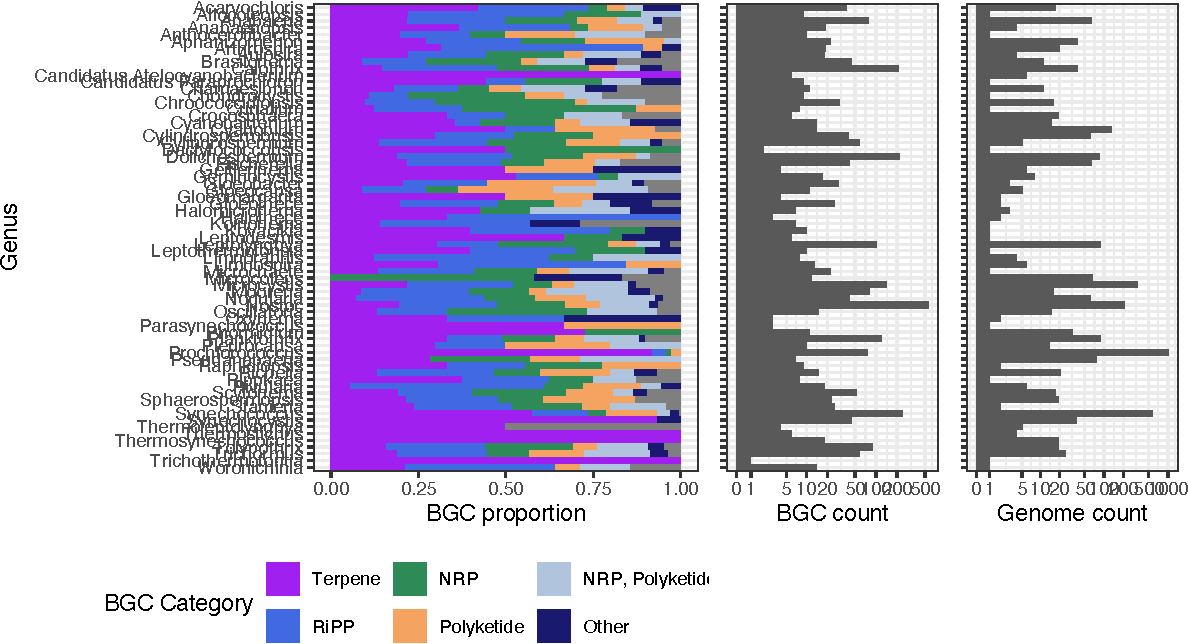
\includegraphics{analysis_files/figure-latex/unnamed-chunk-15-1.pdf}

\begin{Shaded}
\begin{Highlighting}[]
\FunctionTok{ggsave}\NormalTok{(}\StringTok{"./figs/png/split\_triple.png"}\NormalTok{, p5, }\AttributeTok{width =} \DecValTok{8}\NormalTok{, }\AttributeTok{height =} \DecValTok{11}\NormalTok{, }\AttributeTok{device =} \StringTok{"png"}\NormalTok{)}
\end{Highlighting}
\end{Shaded}

\hypertarget{create-figure-2-for-the-manuscript}{%
\subsection{Create Figure 2 for the
manuscript}\label{create-figure-2-for-the-manuscript}}

\begin{Shaded}
\begin{Highlighting}[]
\NormalTok{p\_a }\OtherTok{\textless{}{-}} \FunctionTok{plot\_grid}\NormalTok{(}
\NormalTok{    p\_bgc\_dens }\SpecialCharTok{+} \FunctionTok{theme}\NormalTok{(}\AttributeTok{axis.text.y =} \FunctionTok{element\_text}\NormalTok{(}\AttributeTok{size =} \DecValTok{8}\NormalTok{)), }
\NormalTok{    p\_bgc\_ct, }
\NormalTok{    p\_genome\_ct, }
    \AttributeTok{align =} \StringTok{"h"}\NormalTok{, }
    \AttributeTok{rel\_widths =} \FunctionTok{c}\NormalTok{(}\DecValTok{3}\NormalTok{, }\DecValTok{1}\NormalTok{, }\DecValTok{1}\NormalTok{), }
    \AttributeTok{nrow =} \DecValTok{1}
\NormalTok{    )}

\NormalTok{p\_b }\OtherTok{\textless{}{-}} \FunctionTok{ggplot}\NormalTok{(}
\NormalTok{    region\_summary\_lumped,}
    \FunctionTok{aes}\NormalTok{(}\AttributeTok{y =} \FunctionTok{reorder}\NormalTok{(group, n))}
\NormalTok{) }\SpecialCharTok{+}
  \FunctionTok{geom\_col}\NormalTok{(}\FunctionTok{aes}\NormalTok{(}\AttributeTok{x =}\NormalTok{ n, }\AttributeTok{fill =}\NormalTok{ group)) }\SpecialCharTok{+}
  \FunctionTok{scale\_x\_continuous}\NormalTok{(}\AttributeTok{name =} \StringTok{"BGC count"}\NormalTok{, }\AttributeTok{breaks =} \FunctionTok{breaks\_extended}\NormalTok{()) }\SpecialCharTok{+}
  \FunctionTok{scale\_y\_discrete}\NormalTok{(}\AttributeTok{name =} \StringTok{"BGC Category"}\NormalTok{) }\SpecialCharTok{+}
  \FunctionTok{scale\_fill\_manual}\NormalTok{(}\AttributeTok{values =}\NormalTok{ cat\_colors) }\SpecialCharTok{+}
  \FunctionTok{theme\_bw}\NormalTok{() }\SpecialCharTok{+}
  \FunctionTok{guides}\NormalTok{(}\AttributeTok{fill =} \StringTok{"none"}\NormalTok{)}

\NormalTok{p\_c }\OtherTok{\textless{}{-}}\NormalTok{ regions\_lumped }\SpecialCharTok{\%\textgreater{}\%}
  \FunctionTok{filter}\NormalTok{(group }\SpecialCharTok{!=} \StringTok{"All other hybrids"}\NormalTok{) }\SpecialCharTok{\%\textgreater{}\%}
  \FunctionTok{ggplot}\NormalTok{(}\FunctionTok{aes}\NormalTok{(}\AttributeTok{x =}\NormalTok{ region\_length }\SpecialCharTok{/} \DecValTok{1000}\NormalTok{)) }\SpecialCharTok{+}
      \FunctionTok{geom\_histogram}\NormalTok{(}\FunctionTok{aes}\NormalTok{(}\AttributeTok{fill =}\NormalTok{ group), }\AttributeTok{bins =} \DecValTok{50}\NormalTok{) }\SpecialCharTok{+}
      \FunctionTok{scale\_x\_log10}\NormalTok{(}\AttributeTok{name =} \StringTok{"BGC length (kb)"}\NormalTok{, }\AttributeTok{guide =} \StringTok{"axis\_logticks"}\NormalTok{, }\AttributeTok{limits =} \FunctionTok{c}\NormalTok{(}\DecValTok{1}\NormalTok{, }\ConstantTok{NA}\NormalTok{), }\AttributeTok{breaks =} \FunctionTok{c}\NormalTok{(}\DecValTok{1}\NormalTok{, }\DecValTok{5}\NormalTok{, }\DecValTok{10}\NormalTok{, }\DecValTok{50}\NormalTok{, }\DecValTok{100}\NormalTok{, }\DecValTok{200}\NormalTok{)) }\SpecialCharTok{+}
      \FunctionTok{scale\_y\_continuous}\NormalTok{(}\AttributeTok{name =} \StringTok{"BGC count"}\NormalTok{, }\AttributeTok{breaks =} \FunctionTok{breaks\_extended}\NormalTok{(}\AttributeTok{n =} \DecValTok{3}\NormalTok{)) }\SpecialCharTok{+}
      \FunctionTok{scale\_fill\_manual}\NormalTok{(}\AttributeTok{values =}\NormalTok{ cat\_colors) }\SpecialCharTok{+}
      \FunctionTok{facet\_wrap}\NormalTok{(}\FunctionTok{vars}\NormalTok{(group), }\AttributeTok{ncol =} \DecValTok{1}\NormalTok{, }\AttributeTok{scales =} \StringTok{"free\_y"}\NormalTok{) }\SpecialCharTok{+}
      \FunctionTok{guides}\NormalTok{(}\AttributeTok{fill =} \StringTok{"none"}\NormalTok{) }\SpecialCharTok{+}
      \FunctionTok{theme\_bw}\NormalTok{() }\SpecialCharTok{+}
      \FunctionTok{theme}\NormalTok{(}
        \AttributeTok{strip.background =} \FunctionTok{element\_blank}\NormalTok{(),}
        \AttributeTok{strip.text =} \FunctionTok{element\_blank}\NormalTok{()}
\NormalTok{      )}

\NormalTok{bottom\_row }\OtherTok{\textless{}{-}} \FunctionTok{plot\_grid}\NormalTok{(p\_b, p\_c, }\AttributeTok{nrow =} \DecValTok{1}\NormalTok{, }\AttributeTok{labels =} \FunctionTok{c}\NormalTok{(}\StringTok{"B"}\NormalTok{, }\StringTok{"C"}\NormalTok{), }\AttributeTok{label\_size =} \DecValTok{12}\NormalTok{)}

\NormalTok{fig2 }\OtherTok{\textless{}{-}} \FunctionTok{plot\_grid}\NormalTok{(p\_a, bottom\_row, }\AttributeTok{nrow =} \DecValTok{2}\NormalTok{, }\AttributeTok{labels =} \FunctionTok{c}\NormalTok{(}\StringTok{"A"}\NormalTok{, }\StringTok{""}\NormalTok{), }\AttributeTok{label\_size =} \DecValTok{12}\NormalTok{, }\AttributeTok{rel\_heights =} \FunctionTok{c}\NormalTok{(}\FloatTok{2.5}\NormalTok{, }\DecValTok{1}\NormalTok{))}
\NormalTok{fig2}
\end{Highlighting}
\end{Shaded}

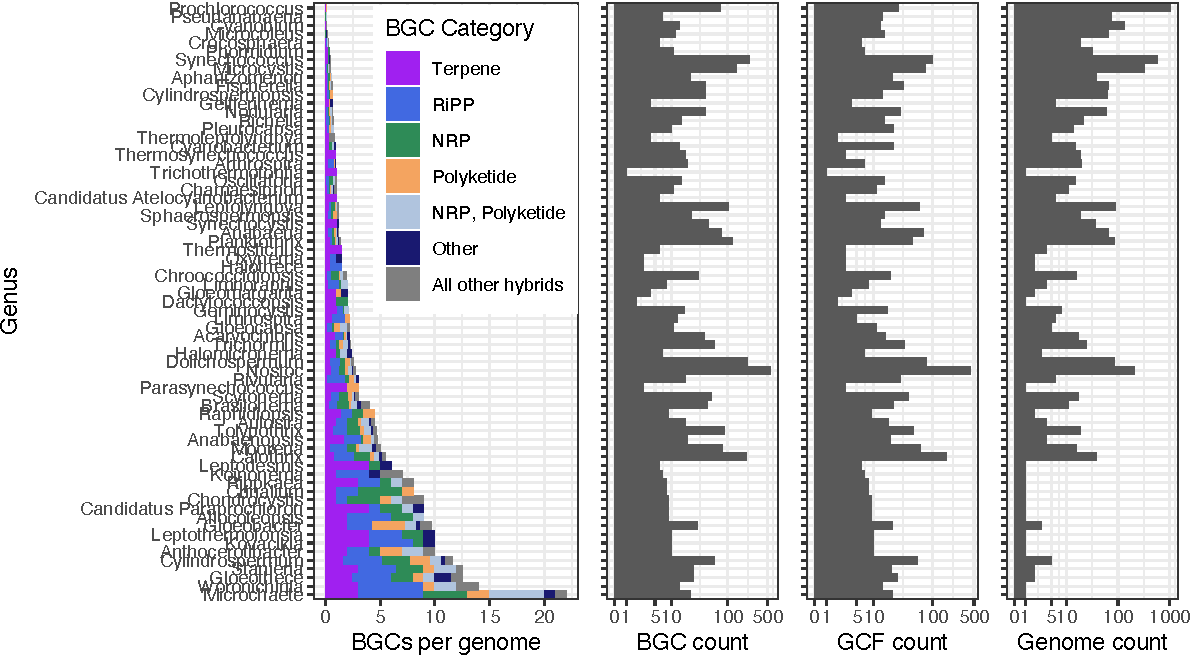
\includegraphics{analysis_files/figure-latex/unnamed-chunk-16-1.pdf}

\begin{Shaded}
\begin{Highlighting}[]
\FunctionTok{ggsave}\NormalTok{(}\StringTok{"./figs/\_fig2.png"}\NormalTok{, fig2, }\AttributeTok{width =} \DecValTok{7}\NormalTok{, }\AttributeTok{height =} \DecValTok{10}\NormalTok{, }\AttributeTok{device =} \StringTok{"png"}\NormalTok{)}
\FunctionTok{ggsave}\NormalTok{(}\StringTok{"./figs/\_fig2.pdf"}\NormalTok{, fig2, }\AttributeTok{width =} \DecValTok{7}\NormalTok{, }\AttributeTok{height =} \DecValTok{10}\NormalTok{, }\AttributeTok{device =} \StringTok{"pdf"}\NormalTok{)}
\end{Highlighting}
\end{Shaded}


\end{document}
